\documentclass[dsc,pdftex]{coppe}
\usepackage[utf8]{inputenc}
\usepackage{amsmath,amssymb, amsfonts}
\usepackage{multirow}
\usepackage{subfigure}
\usepackage{algorithmic}

\usepackage{color}

\makelosymbols
\makeloabbreviations
\newcommand{\wbalTwo}[2][Wikimedia]{
  This is the Wikibook about LaTeX
  supported by {#1} and {#2}!}


\newcommand{\dx}[1][ ]{\frac{\partial {#1}}{\partial x}}
\newcommand{\dy}[1][ ]{\frac{\partial {#1}}{\partial y}}
\newcommand{\dz}[1][ ]{\frac{\partial {#1}}{\partial z}}
\newcommand{\dxi}[1][ ]{\frac{\partial {#1}}{\partial \xi}}
\newcommand{\deta}[1][ ]{\frac{\partial {#1}}{\partial \eta}}
\newcommand{\dzeta}[1][ ]{\frac{\partial {#1}}{\partial \zeta}}

\newcommand{\dxk}[1][ ]{\frac{\partial {#1}}{\partial x_k}}

\newcommand{\Tau}{\mathrm{T}}

\newcommand{\poisson}{\upsilon}

%Deslocamentos

\newcommand{\uvetor}{
\begin{bmatrix}
u_x \\ u_y \\ u_z
\end{bmatrix}
}

%Deformacoes
\newcommand{\exx}{\epsilon_{xx}}
\newcommand{\eyy}{\epsilon_{yy}}
\newcommand{\ezz}{\epsilon_{zz}}
\newcommand{\exy}{\gamma_{xy}}
\newcommand{\exz}{\gamma_{xz}}
\newcommand{\eyx}{\gamma_{yx}}
\newcommand{\eyz}{\gamma_{yz}}
\newcommand{\ezx}{\gamma_{zx}}
\newcommand{\ezy}{\gamma_{zy}}


%Definicao das tensoes efetivas
\newcommand{\sxx}{\sigma^\prime_{xx}}
\newcommand{\syy}{\sigma^\prime_{yy}}
\newcommand{\szz}{\sigma^\prime_{zz}}
\newcommand{\sxy}{\sigma^\prime_{xy}}
\newcommand{\sxz}{\sigma^\prime_{xz}}
\newcommand{\syx}{\sigma^\prime_{yx}}
\newcommand{\syz}{\sigma^\prime_{yz}}
\newcommand{\szx}{\sigma^\prime_{zx}}
\newcommand{\szy}{\sigma^\prime_{zy}}

\newcommand{\evetor}{
\begin{bmatrix}
\exx
\\
\eyy
\\
\ezz
\\
\exy
\\
\exz
\\
\eyz
\end{bmatrix}
}


% Definicao das tensoes totais
\newcommand{\stxx}{\sigma_{xx}}
\newcommand{\styy}{\sigma_{yy}}
\newcommand{\stzz}{\sigma_{zz}}
\newcommand{\stxy}{\sigma_{xy}}
\newcommand{\stxz}{\sigma_{xz}}
\newcommand{\styx}{\sigma_{yx}}
\newcommand{\styz}{\sigma_{yz}}
\newcommand{\stzx}{\sigma_{zx}}
\newcommand{\stzy}{\sigma_{zy}}

\newcommand{\stvetor}{
\begin{bmatrix}
\stxx
\\
\styy
\\
\stzz
\\
\stxy
\\
\stxz
\\
\styz
\end{bmatrix}
}

\newcommand{\stensor}{
\begin{bmatrix}
\stxx & \stxy & \stxz \\
\styx & \styy & \styz \\
\stzx & \stzy & \stzz
\end{bmatrix}
}

\newcommand{\sstensor}{
\begin{bmatrix}
\dx[\stxx] + \dy[\stxy] + \dz[\stxz] \\
\dx[\styx] + \dy[\styy] + \dz[\styz] \\
\dx[\stzx] + \dy[\stzy] + \dz[\stzz]
\end{bmatrix}
}

\newcommand{\Dx}{
\Delta x
}
\newcommand{\Dy}{
\Delta y
}

\newcommand{\Dz}{
\Delta z
}


%Matriz de Elasticidade
\newcommand{\elasticinv}{
\frac{1}{E}
\begin{bmatrix}
        1 & -\upsilon & -\upsilon &             0 &             0 &             0 \\
-\upsilon &         1 & -\upsilon &             0 &             0 &             0 \\
-\upsilon & -\upsilon &         1 &             0 &             0 &             0 \\
        0 &         0 &         0 & 2(1+\upsilon) &             0 &             0 \\
        0 &         0 &         0 &             0 & 2(1+\upsilon) &             0 \\
        0 &         0 &         0 &             0 &             0 & 2(1+\upsilon)
\end{bmatrix}
}


\newcommand{\elastic}{
\frac{E}{(1+\upsilon)(1-2\upsilon)}
\begin{bmatrix}
1 - \upsilon &     \upsilon &     \upsilon &                     0 &                     0 &                     0 \\
    \upsilon & 1 - \upsilon &     \upsilon &                     0 &                     0 &                     0 \\
    \upsilon &     \upsilon & 1 - \upsilon &                     0 &                     0 &                     0 \\
           0 &            0 &            0 & \frac{1-2\upsilon}{2} &                     0 &                     0 \\
           0 &            0 &            0 &                     0 & \frac{1-2\upsilon}{2} &                     0 \\
           0 &            0 &            0 &                     0 &                     0 & \frac{1-2\upsilon}{2}
\end{bmatrix}
}


% Operador S

\newcommand{\sopwithoutb}[1][ ]{
\dx[#1] &        0 &   0      \\
      0 & \dy[#1]  &   0      \\
      0 &        0 & \dz[#1]  \\
\dy[#1] & \dx[#1]  &   0      \\
\dz[#1] &        0 & \dx[#1]  \\
      0 & \dz[#1]  & \dy[#1]
}

\newcommand{\sopnabla}{\nabla_S}

\newcommand{\sop}[1][ ]{
\begin{bmatrix}
\dx[#1] &        0 &   0      \\
      0 & \dy[#1]  &   0      \\
      0 &        0 & \dz[#1]  \\
\dy[#1] & \dx[#1]  &   0      \\
\dz[#1] &        0 & \dx[#1]  \\
      0 & \dz[#1]  & \dy[#1]
\end{bmatrix}
}

\newcommand{\soptwod}[1][ ]{
\begin{bmatrix}
\dx[#1] &        0   \\
      0 & \dy[#1]    \\
\dy[#1] & \dx[#1]    \\
\end{bmatrix}
}

\newcommand{\sopt}[1][ ]{
\begin{bmatrix}
\dx[#1] &       0 &   0     & \dy[#1] & \dz[#1] &   0 \\
      0 & \dy[#1] &   0     & \dx[#1] &       0 & \dz[#1] \\
      0 &       0 & \dz[#1] &       0 & \dx[#1] & \dy[#1]
\end{bmatrix}
}

% Integral em omega

\newcommand{\omeint}[2][\Omega]{\int\limits_{#1} #2 \, d#1}
\newcommand{\omeeint}[1]{\omeint[\Omega^e]{#1}}

\newcommand{\phiix}{\varphi_i(\mathbf{x})}
\newcommand{\phijx}{\varphi_j(\mathbf{x})}

\newcommand{\aepp}[2]{a_e(\varphi_{#1}, \varphi_{#2})}

\newcommand{\aepplocal}[2]{a_e(\varphi^e_{#1}, \varphi^e_{#2})}

\newcommand{\aelinha}[1][i]{\aepp{#1}{1} & \aepp{#1}{2} & \cdots & \aepp{#1}{nn}}

\newcommand{\aelocallinha}[1][i]{\aepplocal{#1}{1} & \aepplocal{#1}{2} & \cdots & \aepplocal{#1}{8}}

\newcommand{\aemat}{
\begin{bmatrix}
\aelinha[1] \\
\aelinha[2] \\
\vdots & \vdots & \ddots & \vdots \\
\aelinha[nn]
\end{bmatrix}}

\newcommand{\aematelem}{
\begin{bmatrix}
\aelocallinha[1] \\
\aelocallinha[2] \\
\vdots & \vdots & \ddots & \vdots \\
\aelocallinha[8] \\
\end{bmatrix}
}

\newcommand{\libvetor}{
 \begin{bmatrix}
  u^{1}_x \\
  u^{1}_y \\
  u^{1}_z \\

  \vdots\\
  u^{nn}_x \\
  u^{nn}_y \\
  u^{nn}_z
 \end{bmatrix}
}



\newcommand{\ldint}[1][i]{(\mathbf{F}, \varphi_{#1})}


%Matrizes Griffiths
\newcommand{\der}{\begin{bmatrix}
\dxi[\phi^1]   & \dxi[\phi^2] & \dxi[\phi^3] & \dxi[\phi^4]      \\
\deta[\phi^1]  & \deta[\phi^2] & \deta[\phi^3] & \deta[\phi^4]    \\
\end{bmatrix}
}

\newcommand{\deriv}{\begin{bmatrix}
\dx[\phi^1]   & \dx[\phi^2] & \dx[\phi^3] & \dx[\phi^4]    \\
\dy[\phi^1]   & \dy[\phi^2] & \dy[\phi^3] & \dy[\phi^4]
\end{bmatrix}
}

\newcommand{\entradaae}[2]{
 (S^T N^{#1})_{x=p_k} D (S N^{#2})_{x=p_k}
}


\newcommand{\preconadd}{
    M^{-1}=M^{-1}_{h} + M^{-1}_{ms}
}

\newcommand{\preconmult}{
    M^{-1}=M^{-1}_{h} + M^{-1}_{ms}(I-K_hM^{-1}_{h})
}

\newcommand{\qtdfreedomfine}{n_u^h}
\newcommand{\essentialfine}{n_{\bar{u}}^h}

\newcommand{\qtdfreedomcoarse}{n_u^H}
\newcommand{\essentialcoarse}{n_{\bar{u}}^H}

\newcommand{\numelementsxfine}{n_x}
\newcommand{\numelementsyfine}{n_y}
\newcommand{\numelementsxcoarse}{n^H_x}
\newcommand{\numelementsycoarse}{n^H_y}


\newcommand{\basefunctionfine}[1][i]{ {\mathbf{N}_{#1}^h} }
\newcommand{\basefunctionelem}[1][i]{ {\mathbf{N}_{#1}^e} }
\newcommand{\basefunctionfineessential}{\mathbf{N}_{i+\qtdfreedomfine}^h}

\newcommand{\basefunctioncoarse}[1][i]{ {\mathbf{N}_{#1}^H} }




\newcommand{\sobolev}{H^1(\Omega)}

\newcommand{\trial}{\mathcal{V}(\Omega)}

\newcommand{\trialaprox}{\mathcal{V}^h}

\newcommand{\trialdef}{\{  \mathbf{w} | \mathbf{w} \in \sobolev ^2 , \mathbf{w} = 0 \text{ em } \Gamma_u \}}

\newcommand{\test}{\mathcal{S}(\Omega)}

\newcommand{\testaprox}{\mathcal{S}^h}

\newcommand{\testdef}{\{  \mathbf{u} | \mathbf{u} \in \sobolev ^2 , \mathbf{u} = \bar{u} \text{ em } \Gamma_u \}}

\newcommand{\qtdnos}{n_{\text{nós}}}

\newcommand{\kij}[2]{(\sopnabla \basefunctionfine[#1])^T D \sopnabla \basefunctionfine[#2]}

\newcommand{\kije}[2]{(\sopnabla \basefunctionelem[#1])^T D \sopnabla \basefunctionelem[#2]}


\newcommand{\intbase}[1]{\int_{-1}^{1}\int_{-1}^{1} #1 d\xi d\eta }

% inicio LMC
\usepackage[draft]{todonotes}   
\newcommand{\suge}[1]{{\bfseries\color{blue}{(sugestão: #1.)\hspace*{5mm}(lmc)}}}
\newcommand{\comen}[1]
{\par {\bfseries \color{magenta} (comentário: #1.) \hspace*{5mm}(lmc)\par}}
\usepackage{fancyvrb}
\usepackage{booktabs}
\usepackage[tableposition=above]{caption} % a distancia entre o caption e a tabela está muito pequena com esse pacote, o problema está resolvido, só que ele dispara alguns warnings, mas todos corretos.

%fim LMC

\begin{document}
  \title{Método Multiescala aplicado à Geomecânica}
  \foreigntitle{geomechanics simulador}
  \author{Mateus}{Oliveira de Figueiredo}
  \advisor{Prof.}{Nelson}{Maculan Filho}{D.Sc.}
  \coadvisor{Prof.}{Luiz Mariano}{Paes de Carvalho Filho}{D.Sc.}
  \examiner{Prof.}{Examinador 1}{D.Sc.}
  \examiner{Prof.}{Examinador 2}{Ph.D.}
  \examiner{Prof.}{Examinador 3}{D.Sc.}
  \department{PESC}
  \date{03}{2019}
  \keyword{Geomecânica}
  \maketitle

  \frontmatter
  %\dedication{A algu\'em cujo valor \'e digno desta dedicat\'oria.}


  %\chapter*{Agradecimentos}

Gostaria de agradecer a todos.

  %\begin{abstract}

Apresenta-se, nesta dissertação, uma aplicação do método mutiescala para o problema Geomecânico de Elasticidade linear. A aplicação consiste em utilizar um pré-condicionador multiescala junto com um pré-condicionador no espaço fino para reduzir o número de iterações de solvers lineares como o Gradiente Conjugado e Bicgstab. Os resultados mostram comparações entre a utilização de pré-condicionadores acoplados de maneira aditiva e de forma multiplicativa mostrando que em casos que o engrossamento é suficientemente alto a redução da complexidade do aditivo pode trazer ganho nos tempos de solução. Além disso, é mostrada uma comparação com o solver multigrid sendo ambos os solvers utilizados como precondicionador para o gradiente conjugado. 

\end{abstract}


  %\begin{foreignabstract}

In this work, we present ...

\end{foreignabstract}


  \tableofcontents
  \listoffigures
  \listoftables
  \printlosymbols
  \printloabbreviations

  \mainmatter

  \chapter{Introdução}

  \chapter{Modelagem Matemática} \label{ch:modelagem}
  
Nesse capítulo, serão apresentados as equações que regem os fenômenos geomecânicos. O primeiro trabalho famoso na modelagem de tensões no solo é Terzaghi que desenvolveu a teoria para uma dimensão. Mais tarde, Biot generalizou essa teoria para três dimensões e essas são as equações que serão apresentadas. Detalhes das duas teorias podem ser encontradas em \citet{CompGeomec}. Como o intuito do trabalho é avaliar o método multiescala aplicado para matrizes dessa natureza, o caso aqui considerado será o de elasticidade linear onde a rocha não é tensionada até que apresente falhas.



\section{Tensor de Tensões}

Para representar a tensão total em um ponto da rocha, é utilizado um tensor de tensões de segunda ordem como mostra \eqref{eq:tensordetensoes}.

\begin{equation} \label{eq:tensordetensoes}
\mathbf{\st} =
    \begin{bmatrix}
    \stxx & \stxy & \stxz \\
    \styx & \styy & \styz \\
    \stzx & \stzy & \stzz
    \end{bmatrix}
\end{equation}

O primeiro subscrito do tensor representa a face que a tensão está sendo aplicada, enquanto o segundo representa a direção da tensão. A Figura \ref{fig:tensoesx} mostra as componentes com o com primeiro subscrito $x$.


\begin{figure}[!htbp]
\centering
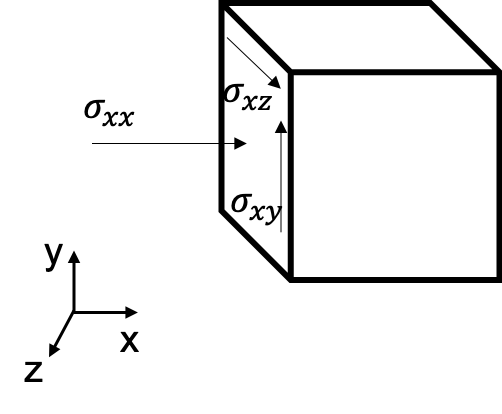
\includegraphics[width=5cm]{chap01/figs/tensor.png}
\caption{Tensões $\sigma_{x.}$ representadas graficamente.}
\label{fig:tensoesx}
\end{figure}

Ao aplicar a condição de equilíbrio do momento, chega-se a conclusão que $\stxy=\styx$, $\stxz=\stzx$ e $\styz=\stzy$. Dessa maneira, para a representação desse tensor, são necessários guardar apenas seis valores. Pode-se considerar então a tensão como o vetor apresentado \eqref{eq:tensor6} essa notação é chamada de notação de Voigt e é a bastante utilizada nas implementações de elementos finitos, por exemplo, nas formulações apresentadas por \citet{hughes} e \citet{jacob}.


\begin{equation}
\st^T = \begin{bmatrix}
\stxx & \styy & \stzz & \stxy & \stxz & \styz
\end{bmatrix}
\label{eq:tensor6}
\end{equation}


\section{Teoria da Consolidação}

Para um certo elemento de volume $\Delta x\Delta y \Delta z$ pode-se escrever as equações de equilíbrio para cada uma dessas direções. A Figura \ref{fig:equilibrio} apresenta todas as tensões relativas à direção x.

\begin{figure}[!htbp]
\centering
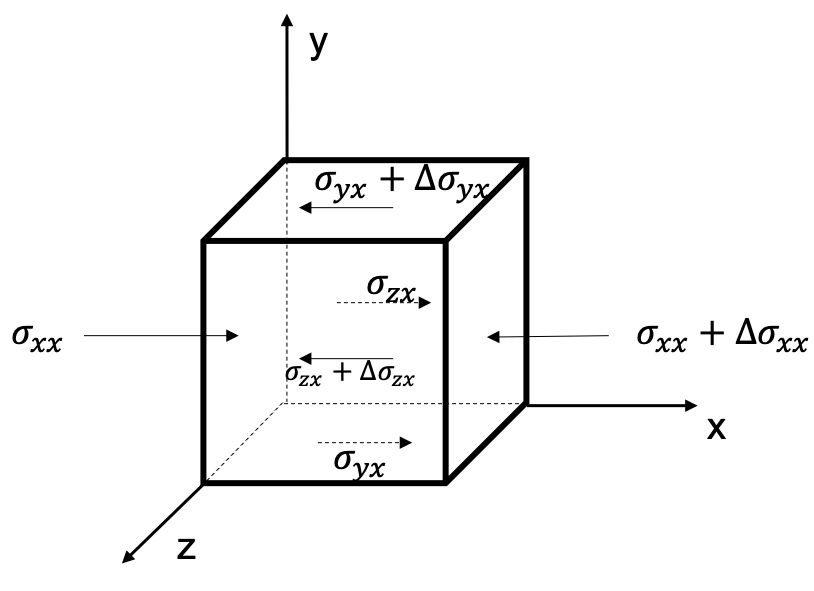
\includegraphics[width=8cm]{chap01/figs/equilibrio.png}
\caption{Tensões na direção x ($\sigma_{.x}$) representadas graficamente.  Adaptado de \cite{CompGeomec}.}
\label{fig:equilibrio}
\end{figure}


As forças atuantes no cubo são calculadas a partir da tensão multiplicada pela área de atuação. Sobre o valor $f_x$, ele, juntamente com os termos $f_y$ e $f_z$  são termos gravitacionais e representam a força peso do volume $\Dx\Dy\Dz$. Como apresentado em \citet{xiuligai}, $\mathbf{f} = [\rho_s(1-\phi) + \phi(\rho_o S_o + \rho_w S_w + \rho_g S_g )] \mathbf{g}$ onde $\phi$ é a porosidade, $S_o$, $S_w$ e $S_g$ as saturações de óleo, água e gás e $\rho_o$, $\rho_w$, $\rho_g$, $\rho_s$  as densidades do óleo, água, gás e rocha e $\mathbf{g}$ o vetor gravidade. O termo gravitacional será considerado constante ao longo da simulação, fazendo com que as modificações no equilíbrio sejam apenas relativas à mudança de pressão. 

O equilíbrio de forças na direção x pode ser escrito como apresentado em \eqref{eq:equilibrio0}. 


\begin{multline} \label{eq:equilibrio0}
   (\stxx - \stxx - \Delta \stxx) \Dy\Dz + (\styx - \styx - \Delta \styx)\Dx\Dz  +\\
   + (\stzx - \stzx - \Delta\stzx) \Dx\Dy + f_x\Dx\Dy\Dz = 0
\end{multline}


\begin{equation}
 \Delta \stxx \Dy\Dz + \Delta \styx\Dx\Dz + \Delta\stzx \Dx\Dy - f_x\Dx\Dy\Dz = 0
\end{equation}

Dividindo todos os termos por $\Dx\Dy\Dz$.


\begin{equation}
\frac{ \Delta \stxx }{ \Dx } + \frac{\Delta \styx}{ \Dy } + \frac{\Delta\stzx}{ \Dz } - f_x = 0
\end{equation}

Fazendo $\Dx \rightarrow 0$, $\Dy \rightarrow 0 $ e $\Dz \rightarrow 0$

\begin{equation}
\dx[\stxx] + \dy[\styx] + \dz[\stzx] - f_x = 0
\end{equation}

Analogamente, para as direções y e z pode-se encontrar a equação de equilíbrio também, montando o sistema \eqref{eq:equilibrio1}.

\begin{equation}
\label{eq:equilibrio1}
\left\{\begin{matrix}
 \dx[\stxx] + \dy[\styx] + \dz[\stzx] - f_x & = & 0\\
 \dx[\stxy] + \dy[\styy] + \dz[\stzy] - f_y & = & 0\\
 \dx[\stxz] + \dy[\styz] + \dz[\stzz] - f_z & = & 0
\end{matrix}\right.
\end{equation}


As tensões apresentadas em \eqref{eq:equilibrio1} são as tensões totais que atuam no cubo infinitesimal. Acontece que, como mostra a Figura \ref{fig:rochaComFluido}, os reservatórios de petróleo possuem fluído no volume poroso da rocha (óleo, água e gás) e, portanto, parte da tensão total será suportada pelo fluído e parte será suportada pelos grãos da rocha. Como o fluído não oferece resistência ao cisalhamento, ele suporta apenas a parte das tensões $\stxx$, $\styy$ e $\stzz$.

\begin{figure}[!htbp]
\centering
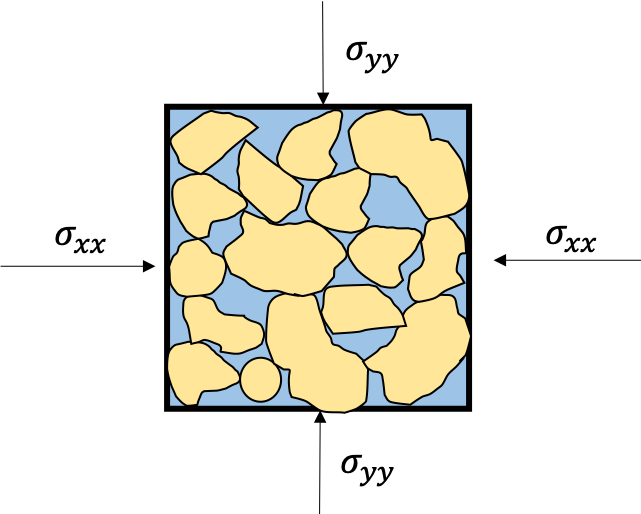
\includegraphics[width=7cm]{chap01/figs/fluido_rocha_tensoes.png}
\caption{Representação de meio poroso. Grãos amarelos representando a matriz da rocha e fluído representado pela cor azul.}
\label{fig:rochaComFluido}
\end{figure}

Conforme mostrado pela teoria da consolidação de poroelasticidade, desenvolvida por Biot para três dimensões, a tensão efetiva na rocha ($\stef$) e a tensão total são relacionadas por \eqref{eq:tensaoefetiva}, conforme mostrado em \citet{ResGeomec}.


\begin{equation}
\label{eq:tensaoefetiva}
\left\{\begin{matrix}
 \sxx = \stxx - \alpha P_p \\
 \syy = \styy - \alpha P_p \\
 \szz = \stzz - \alpha P_p
\end{matrix}\right.
\end{equation}


Onde $\sxx$, $\syy$  e $\szz$ são as tensões efetivas, $\alpha$ é o coeficiente de Biot e $P_p$ a pressão de poros. O coeficiente de Biot representa o quanto a pressão de poros do fluído suporta a tensão total na rocha e está no intervalo $\alpha \in [0,1]$.

As equações \eqref{eq:equilibrio1} podem ser reescritas como \eqref{eq:equilibrio} substituindo as tensões totais ($\st$) pela tensões efetivas na rocha ($\stef$).

\begin{equation}
\label{eq:equilibrio}
\left\{\begin{matrix}
\dx[\sxx]  + \dy[\syx] + \dz[\szx] - \dx[\alpha P_p] - f_x   = 0
\\
\dx[\sxy]  + \dy[\syy] + \dz[\szy] - \dy[\alpha P_p] - f_y   = 0
\\
\dx[\sxz]  + \dy[\syz] + \dz[\szz] - \dz[\alpha P_p] - f_z   = 0
\end{matrix}\right.
\end{equation}

Ou ainda, escrevendo \eqref{eq:equilibrio} utilizando os operadores divergente, gradiente e $\mathbf{f}^T=\begin{bmatrix}f_x & f_y & f_z\end{bmatrix}$ pode-se chegar em
\eqref{eq:equilibrio_matriz}.

\begin{equation}
\label{eq:equilibrio_matriz}
\nabla \cdot \stef - \nabla \cdot \alpha \mathbf{I} P_p - \mathbf{f} = 0
\end{equation}

Por motivos de implementação mais eficiente, menor uso de memória e utilização de operações mais simples (multiplicação de matrizes por vetores), a Equação \eqref{eq:equilibrio_matriz} pode ser escrita na notação de Voigt considerando as definições conforme \eqref{eq:definicoesvoigt}.

\begin{equation}
\label{eq:equilibrio_final}
\sopnabla^T \stef - \sopnabla^T\alpha \mathbf{m}  P_p - \mathbf{f} = 0
\end{equation}

Onde,
\begin{equation}
\begin{matrix}\label{eq:definicoesvoigt}
\stef = \begin{bmatrix}
\sxx
\\
\syy
\\
\szz
\\
\sxy
\\
\sxz
\\
\syz
\end{bmatrix}
&

;

&

\mathbf{f} = \begin{bmatrix}
f_{x}
\\
f_{y}
\\
f_{z}
\end{bmatrix}
&
;
&

\mathbf{m} = \begin{bmatrix} 1 \\ 1 \\ 1 \\ 0 \\ 0 \\ 0\end{bmatrix}

&
;

&
\sopnabla = \sop
\end{matrix}
\end{equation}



\subsection{Relações Constitutivas}

A Equação \eqref{eq:equilibrio_final} apresenta o equilíbrio em função das tensões. Porém, pelo grande número de variáveis dessa equação, é necessário colocar em função das variáveis de deslocamento para que seja possível resolve-la. O campo de deslocamentos será representado pela variável $\deslocamento = [u_x \quad u_y \quad u_z]^T$. A deformação ($\deformacao$) se relaciona com o deslocamento de acordo com \eqref{eq:defor_desloc}. 

\begin{equation}
\label{eq:defor_desloc}
\deformacao = \sopnabla \deslocamento
\end{equation}


Já a relação entre a deformação e as tensões é definida como relação constitutiva de acordo com \citet{ResGeomec}. Diferentes tipos de relações constitutivas podem ser utilizadas para representar essa relação entre tensão e deformação. A Figura \ref{fig:stress_strain} mostra dados de um teste típico de tensão-deformação em uma rocha bem cimentada. Nesse caso, é importante notar que existe um comportamento linear dominante na parte central do gráfico antes da falha. Essa região onde as deformações e tensões se relacionam linearmente é chamada de elástica, e será a região de estudo desse trabalho. 


\begin{figure}[!htbp]
\centering
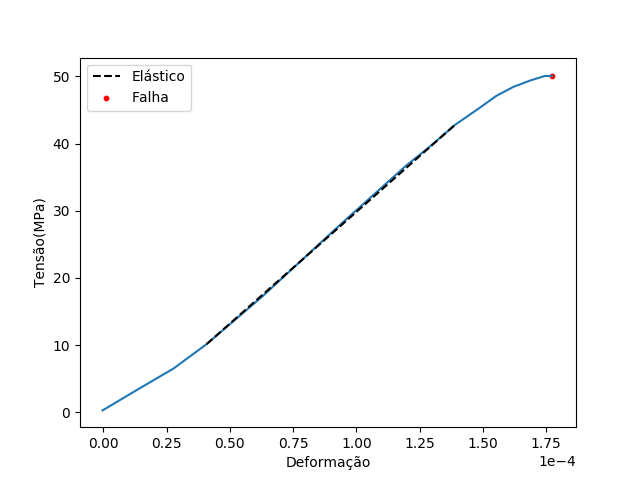
\includegraphics[width=8cm]{chap01/figs/stress_strain.png}
\caption{Teste de laboratório tensão-deformação para uma rocha bem cimentada. Adaptada de \citet{ResGeomec}.}
\label{fig:stress_strain}
\end{figure}


Para o caso de elasticidade linear, a relação entre tensões e deformação é dada por uma forma simples  que é a Lei de Hooke Generalizada apresentada em \eqref{eq:hooke}. Essa equação é a mesma que apresentada a para estudos de mecânica dos sólidos clássicos.

\begin{equation}{
\label{eq:hooke}
\stef = \mathbf{D} \deformacao
}
\end{equation}


\begin{equation}\label{eq:ddefinition}
    \mathbf{D} = \frac{E}{(1+\upsilon)(1-2\upsilon)} \begin{bmatrix}
    1-\upsilon & \upsilon    &  \upsilon & 0 & 0 & 0     \\
      \upsilon &  1-\upsilon &  \upsilon & 0 & 0 & 0     \\
      \upsilon & \upsilon   &  1-\upsilon &  0 & 0 & 0   \\
    0& 0& 0 & \frac{1-2\upsilon}{2} & 0 & 0              \\
    0& 0& 0 & 0 &\frac{1-2\upsilon}{2} & 0               \\
    0& 0& 0 & 0 & 0 &  \frac{1-2\upsilon}{2}             \\
\end{bmatrix}
\end{equation}

onde, $E$ é o módulo de Young e $v$ o módulo de Poisson da rocha.


A EDP da equação \eqref{eq:equilibrio_final} pode então ser escrita em função dos deslocamentos, inserindo \eqref{eq:defor_desloc} e \eqref{eq:hooke} em  \eqref{eq:equilibrio_final}.

\begin{equation}
\label{eq:edp_geomec}
\sopnabla^T \mathbf{D} \sopnabla \deslocamento - \sopnabla^T\alpha \mathbf{m} P_p - \mathbf{f} = 0
\end{equation}

 Essa forma será a utilizada junto dos métodos do elementos finitos para construção de um simulador para regime permanente de geomecânica em duas dimensões. Ao se passar \eqref{eq:edp_geomec} de três dimensões para duas existem duas abordagens possíveis: tensão plana ou deformação plana. As matrizes de elasticidade são apresentadas respectivamente em \eqref{eq:elasticplanestress} e \eqref{eq:elasticplanestrain}.

\begin{equation} \label{eq:elasticplanestress}
\mathbf{D}_{stress} = \frac{E}{1-\upsilon^2}
\begin{bmatrix}
1  & \upsilon & 0 \\
\upsilon & 1 &  0 \\
0 & 0 & \frac{1-\upsilon}{2}
\end{bmatrix}
\end{equation}

\begin{equation} \label{eq:elasticplanestrain}
\mathbf{D}_{strain} = \frac{E}{(1+\upsilon)(1-2\upsilon)}
\begin{bmatrix}
 1-\upsilon & \upsilon    &  0 \\
 \upsilon   &  1-\upsilon &  0 \\
 0& 0 & \frac{1-2\upsilon}{2}
\end{bmatrix}
\end{equation}

De acordo com \citet{jacob}, a condição de deformação plana é melhor aplicada quando o elemento é grosso em relação ao plano xy , que é o caso dos reservatórios de petróleo com os mesmos eixos definidos na Figura \ref{fig:equilibrio}. Dessa forma, artigos como \cite{casteletto}, \cite{planeStrainProblems} e \cite{irina} utilizam a hipótese de deformação plana que é a mesma utilizada nessa dissertação. Os operadores e vetores podem ser redefinidos para os mostrados em \eqref{eq:vetores2d}.

\begin{equation}
\label{eq:vetores2d}
\begin{matrix}
\stef = \begin{bmatrix}
\sxx
\\
\syy
\\
\sxy
\end{bmatrix}
&

;

&

\mathbf{f} = \begin{bmatrix}
f_{x}
\\
f_{y}
\end{bmatrix}
&
;
&

\mathbf{m} = \begin{bmatrix} 1 \\ 1 \\ 0\end{bmatrix}

&
;

&
\sopnabla = \soptwod

&
;

&

\deslocamento = \begin{bmatrix}
u_x
\\
u_y
\end{bmatrix}

\end{matrix}
\end{equation}

Além de \eqref{eq:edp_geomec}, são necessárias as condições de contorno para que o problema fique totalmente definido. Existem dois principais tipos de condição de contorno a de Dirichlet, onde o deslocamento da fronteira é prescrito e condição de contorno de Neumann, onde a tensão normal a fronteira é prescrita. Considerando $\Omega$ o domínio em que está sendo resolvido o problema e $\Gamma = \partial \Omega$ a fronteira do domínio, pode-se dividi-la em duas partes $\Gamma_u$ e $\Gamma_{\sigma}$, onde $\Gamma_u \cup \Gamma_{\sigma} = \Gamma$, $\Gamma_u \cap \Gamma_{\sigma} = \emptyset$, que possuem condição de Dirichlet e Neumann respectivamente. O problema fica então totalmente definido em \eqref{eq:edp_geomec_contorno}.


\begin{equation} \label{eq:edp_geomec_contorno}
\begin{aligned}
     \sopnabla^T \mathbf{D} \sopnabla \deslocamento - \sopnabla^T\alpha \mathbf{m} P_p - \mathbf{f} = 0, & \text{ em }\Omega  \\
     \deslocamento = \bar{\mathbf{u}},& \text{ em } \Gamma_u \\
    \begin{bmatrix}
        \stxx^{\prime\prime} & \stxy^{\prime\prime}
    \end{bmatrix} \mathbf{n} = \bar{t}_x \text{   }     \begin{bmatrix}
        \stxy^{\prime\prime} & \styy^{\prime\prime}
    \end{bmatrix} \mathbf{n} = \bar{t}_y, & \text{   em } \Gamma_{\sigma} 
\end{aligned}  
\end{equation}
onde, $\mathbf{n}$ representa o vetor normal a $\Gamma$, $\bar{\deslocamento} \in \mathbb{R}^2$ e $\bar{\mathbf{t}} = [ \bar{t}_x \quad \bar{t}_y ]$. O problema \eqref{eq:edp_geomec_contorno} pode ser descrito mais genericamente com regiões da fronteira onde uma condição de contorno de Dirichlet é aplicada apenas ao campo $u_x$ ou $u_y$ enquanto o outro campo tem condição de Neumann. Esse exemplo mais geral pode ser encontrado em \citet{hughes}.


  \chapter{Discretização} \label{ch:discretizacao}

  \chapter{Simulação Geomecânica}

  Nesse capítulo, ...

  \chapter{Solução de Sistemas Lineares}\label{ch:sistemas}
  

Nesse capítulo, serão mostrados as técnicas utilizadas para a solução dos sistemas lineares gerados a partir da discretização apresentada no Capítulo \ref{ch:discretizacao}. Nas simulações reais de geomecânica, a quantidade de células pode chegar a centenas de milhões de elementos de forma que métodos efetivos de estruturas de dados e algoritmos são necessários para que a resolução seja possível. A Seção \ref{sec:csr} apresenta uma breve discussão sobre as estruturas de dados para armazenamento das matrizes, a Seção \ref{sec:cg} apresenta alguns métodos de solução de sistemas esparsos, enquanto que a Seção \ref{sec:fatoracaolu} apresenta a fatoração LU.


\section{Estruturas de Dados para Matrizes Esparsas} \label{sec:csr}

Conforme mostrado no Capítulo \ref{ch:discretizacao}, a quantidade de não zeros da matriz (nnz) é $O(\qtdnos)$, enquanto a quantidade total de entradas da matriz é da ordem de $O(\qtdnos^2)$. Dessa forma, é necessário utilizar uma estrutura de dados que seja capaz de  armazenar apenas os não zeros para tornar o \textit{software} mais eficiente.  Uma ideia simples para guardar esse tipo de matriz consiste em guardar para cada elemento não zero seu valor, sua linha e sua coluna. Esse formato é chamado de \textit{Coordinate Format} (COO) mostrado em \citet{solverlinear}. Três vetores são necessários para guardar os valores:


\begin{itemize}
    \item JR: vetor que guarda a linha de cada entrada (Tamanho $nnz$)
    \item JC: vetor que guarda a coluna de cada entrada (Tamanho $nnz$)
    \item AA: vetor que guarda os valores das entrada (Tamanho $nnz$)
\end{itemize}


Assim a matriz


\begin{equation}
    \begin{bmatrix}
        1 & 0 & 2 & 0\\
        3 & 4 & 0 & 5\\
        0 & 6 & 7 & 0\\
        0 & 0 & 8 &9
    \end{bmatrix}
\end{equation}

Tem como vetores associados na sua representam COO os mostrados abaixo:


\begin{center}
    \begin{itemize}
        \item  JR = 1 1 2 2 2 3 3 4 4
        \item  JC = 1 3 1 2 4 2 3 3 4
        \item  AA = 1 2 3 4 5 6 7 8 9
    \end{itemize}
\end{center}


É importante perceber que nesse formato, as entradas da matriz podem ser escritas em qualquer ordem. Porém, no exemplo acima, elas estão ordenadas por linha e pode-se notar que o vetor JR apresenta uma série de valores repetidos. Para tirar proveito dessa repetição, existe outro formato chamado \textit{Compressed Sparse Row Format} (CSR) onde o vetor associado as linhas JR é substituido por um vetor IA que é um ponteiro para o vetor de colunas com o início de cada uma das linhas.

Para a matriz acima, tem-se:

\begin{itemize}
    \item A linha 1 é a primeira e, portanto, IA(1) = 1
    \item A linha 2 começa a partir do elemento 3 do vetor AA e, portanto, IA(2) = 3
    \item A linha 3 começa a partir do elemento 5 do vetor AA e, portanto, IA(3) = 6
    \item A linha 4 começa a partir do elemento 7 do vetor AA e, portanto, IA(4) = 8
\end{itemize}

É adicionado ainda um valor a mais ao vetor IA que guarda a quantidade de nnz+1, no exemplo acima, esse valor é IA(5) = 10. Com isso é possível saber as entradas de determinada linha $i$ olhando para as posições IA(i) a IA(i+1)-1 do vetor AA e as respectivas colunas em JC. Os valores dos vetores CSR da matriz então ficam:

%TODO deixar valores one-based
\begin{center}
    \begin{itemize}
        \item IA = 1 3 7 8 10
        \item JC = 1 3 1 2 4 2 3 3 4
        \item AA = 1 2 3 4 5 6 7 8 9
    \end{itemize}
\end{center}


De acordo com \citet{solverlinear}, o formato CSR é provavelmente o mais comum para guardar matrizes esparsas e costuma ser a porta de entrada de estrutura de dados para matrizes esparsas. Nesse trabalho, a implementação é feita utilizando esse tipo de estrutura de dados conforme será mostrado no Capítulo \ref{ch:implementacao}.

Uma operação particularmente importante com matrizes é a multiplicação matriz vetor $\mathbf{y} = \mathbf{A}\mathbf{x}$. No contexto dessa dissertação, ela é importante para aplicar o operadores de prolongamento e restrição apresentados no Capítulo \ref{ch:multiescala} e também nos métodos iterativos de solução de sistemas lineares: Gradiente Conjugado (CG) e Bicgstab. O Algoritmo \ref{alg:algoritmomatmult} apresenta a multiplicação matriz vetor utilizando uma matriz CSR representada pelos vetores IA, JC, AA pelo vetor x.


\vspace{1cm}
\begin{algorithm}[H]
\caption{y = MultMatrizVetor(IA(n+1), JC(nnz), AA(nnz), x(n))}
\label{alg:algoritmomatmult}
\Inicio{

 y $\leftarrow \mathbf{0}$ 
 
\Para{row $\in$ \{1, 2, 3, ..., n\}}{
    \Para{j $\in$ \{IA(\text{row}), ..., IA(\text{row}+1)-1\}}{
        col $\leftarrow$ JC(j)
        
        y(row) $\leftarrow$ y(row) + AA(j) $\times$ x(col)
    }
}

}

\end{algorithm}
\vspace{1cm}


Nesse algoritmo, é importante perceber que a variável j irá assumir valores de 1 a IA(n+1)-1 e , como IA(n+1)=$\text{nnz} + 1$, a multiplicação tem que complexidade $O(\text{nnz})$. O CSR então, além de necessitar de menos memória para armazenar a matriz, também tem a vantagem de fazer operações de multiplicação mais eficientemente visto que a complexidade seria $O(n^2)$ caso a matriz fosse armazenada densa.


\section{Solução de Sistemas Esparsos} \label{sec:cg}

Nessa seção serão apresentados alguns métodos para solução de sistemas lineares, em especial o Gradiente Conjugado que será utilizado para as comparações entre o método multiescala e multigrid apresentados no Capítulo \ref{ch:resultados}. Será considerado o sistema linear apresentado em \eqref{eq:sistemalinear4}.

\begin{equation} \label{eq:sistemalinear4}
    \mathbf{Ax = b}
\end{equation}

\subsection{Precondicionadores}

Define-se como número de condicionamento da matriz a equação apresentada em \eqref{eq:condicionamento}, quanto maior esse valor mais difícil a convergência do sistema com métodos de Krylov. As matrizes advindas de sistemas gerados por \eqref{eq:edp_geomec_contorno} costumam ter números de condicionamentos elevados fazendo com que os métodos de solução tenham dificuldade de convergir.

\begin{equation} \label{eq:condicionamento}
\text{cond}(\mathbf{A}) = || \mathbf{A} || \cdot || \mathbf{A}^{-1} ||
\end{equation}


Uma estratégia importante para a solução desses sistemas lineares é a utilização de precondicionadores que consistem em tentar resolver um sistema equivalente a \eqref{eq:sistemalinear4} mas com um número de condicionamento menor. Há dois principais métodos de precondicionamento, pela esquerda ou pela direita. Chamando de $\mathbf{M}$ a matriz de precondicionamento, \eqref{eq:preconesq} e \eqref{eq:precondir} apresentam o precondicionamento pela esquerda e pela direita respectivamente. Também é possível fazer o precondicionamento utilizando ambos os lados. A matriz de precondicionamento geralmente aproxima a matriz original $\mathbf{A}$, de forma que $\precon \mathbf{A}$ e $\mathbf{A} \precon$ tenham número de condicionamento ordens de grandeza menores que o da matriz original. Um fato importante é que, apesar de aparecerem os produtos $\precon \mathbf{A}$ e $\mathbf{A} \precon$, eles não efetivamente realizados, pois, muitas vezes se é conhecido apenas a matriz $\mathbf{M}$ e, mesmo que $\precon$ fosse conhecido, esses produtos podem ser densos.  


\begin{equation} \label{eq:preconesq}
\precon \mathbf{A} \mathbf{x}= \precon \mathbf{b}
\end{equation}

\begin{align} \label{eq:precondir}
\mathbf{A} \precon \mathbf{y} = \mathbf{b} \\
\mathbf{x} = \precon \mathbf{{y}}
\end{align}


Precondicionadores populares são os baseados em fatorações incompletas (ILU) apresentados em \citet{ilupaper}. Esses precondicionadores calculam aproximações para a fatoração LU de uma matriz e são apresentadas na seção \ref{sec:fatoracaolu}.

\subsection{Iteração de Richardson}

Um método simples de solução de sistemas lineares é a Iteração de Richardson, essa solução é utilizado em solvers multiescala apresentados em \citet{msparalelo}. No caso, dada a matriz uma matriz $\mathbf{A}$ e um precondicionador $\mathbf{M}$ uma iteração do método é definida conforme apresentado em \eqref{eq:iteracaorichardson}.

\begin{align} \label{eq:iteracaorichardson}
\mathbf{I}_m = (\mathbf{I} - \precon \mathbf{A})    \\
\mathbf{x}_{i+1} = \mathbf{I}_m  \mathbf{x}_i + \precon \mathbf{b}  
\end{align}

Onde, $\mathbf{I}$ representa a matriz identidade. A partir de \eqref{eq:iteracaorichardson} é possível encontrar a equação do erro ao longo das iterações $e_{i+1} = \mathbf{I}_m e_i$, isso faz com que a convergência seja garantida apenas se $\rho(\mathbf{I}_m) < 1$, onde $\rho$ representa o raio espectral da matriz. Essa condição é necessária para que cada componente do erro relativa a cada  um dos autovetores reduza a cada iteração.


\subsection{Método do Gradiente Conjugado}

O método do Gradiente Conjugado pode ser utilizado na solução de sistemas lineares da forma \eqref{eq:sistemalinear4} onde $\mathbf{A}$ é uma matriz simétrica positiva definida (SPD). Nesse caso, pode-se encontrar um problema de minimização equivalente através da definição da forma quadrática apresentada em \eqref{eq:quadratica}. 

\begin{equation} \label{eq:quadratica}
    f(\mathbf{x}) = \frac{1}{2}  \mathbf{x}^T \mathbf{A} \mathbf{x} - \mathbf{b}^T \mathbf{x} + c, \quad f:\mathbb{R}^n \rightarrow \mathbb{R}
\end{equation}

Para encontrar os pontos extremos da função \eqref{eq:quadratica} é necessário calcular os pontos em que o gradiente de $f$ é o vetor nulo. Portanto, é necessário calcular a derivada parcial de $f$ para cada uma das coordenadas. Para facilitar esse cálculo a equação \eqref{eq:quadratica} é apresentada em notação indicial em \eqref{eq:quadratica_ind}.


\begin{equation} \label{eq:quadratica_ind}
    f(\mathbf{x}) = \frac{1}{2} x_i A_{ij} x_j - b_i x_i + c_i
\end{equation}


Aplicando a derivada parcial com relação a uma coordenada $x_k$.


\begin{eqnarray}
     \dxk[f(\mathbf{x})] & = & \frac{1}{2} \dxk[ x_i A_{ij} x_j ]- \dxk{b_i x_i}+ \dxk{c_i} \\
                & = & \frac{1}{2} \dxk[ x_i A_{ij} x_j ]- b_k \\
                & = & \frac{1}{2} (\dxk[ x_i ]A_{ij} x_j  + x_i A_{ij} \dxk[x_j]) - b_k \\
                & = & \frac{1}{2}(A_{kj} x_j  + x_i A_{ik})  - b_k
\end{eqnarray}


Retornando para a notação matricial


\begin{equation}
    \nabla f = \frac{1}{2} (\mathbf{A}\mathbf{x} + \mathbf{A}^T \mathbf{x}) - \mathbf{b}
\end{equation}


\begin{equation}
    \nabla f = \frac{1}{2} (\mathbf{A} + \mathbf{A}^T) \mathbf{x} - \mathbf{b}
\end{equation}

Como $\mathbf{A}$ é simétrica ($\mathbf{A}^T = \mathbf{A}$)

\begin{equation} \label{eq:gradf}
    \nabla f = \mathbf{A} \mathbf{x} - \mathbf{b}
\end{equation}

Em um ponto extremo  $ \mathbf{x}_e$ de $f(\mathbf{x})$ tem-se $(\nabla f)|_{\mathbf{x}=\mathbf{x}_e} = 0 $

\begin{equation}
    \mathbf{A}\mathbf{x}_e - \mathbf{b} = 0
\end{equation}

\begin{equation}
    \mathbf{A}\mathbf{x}_e = \mathbf{b}
\end{equation}

Portanto, $f(\mathbf{x})$ possui um único ponto extremo $\mathbf{x}_e = \mathbf{A}^{-1}\mathbf{b}$ que é justamente a solução do sistema linear \eqref{eq:sistemalinear4}. Resta mostrar que $\mathbf{x}_e$ é um ponto de mínimo. A demonstração a seguir pode ser encontrada em \citet{Shewchuk94anintroduction}. Considerando $\mathbf{x} = \mathbf{x}_e + \mathbf{e}$ com $\mathbf{e} \neq 0 $


\begin{align}
     f(\mathbf{x}_e + \mathbf{e}) & =  \frac{1}{2} (\mathbf{x}_e + \mathbf{e})^T \mathbf{A} (\mathbf{x}_e + \mathbf{e}) - \mathbf{b}^T(\mathbf{x}_e + \mathbf{e}) + \mathbf{c}  \nonumber\\
                & =  \frac{1}{2} (\mathbf{x}_e^T\mathbf{A}\mathbf{x}_e + \mathbf{x}_e^T\mathbf{A}\mathbf{e} + \mathbf{e}^T\mathbf{A}\mathbf{x}_e + \mathbf{e}^T\mathbf{A}\mathbf{e} )- \mathbf{b}^T(\mathbf{x}_e + \mathbf{e}) + \mathbf{c}  \nonumber\\
                & =  \frac{1}{2} \mathbf{x}_e^T\mathbf{A}\mathbf{x}_e -\mathbf{b}^T\mathbf{x}_e + \mathbf{c} + \frac{1}{2} ( \mathbf{x}_e^T\mathbf{A}\mathbf{e} + \mathbf{e}^T\mathbf{A}\mathbf{x}_e + \mathbf{e}^T\mathbf{A}\mathbf{e} ) - \mathbf{b}^T\mathbf{e}  \nonumber\\
                & =  f(\mathbf{x}_e) + \frac{1}{2} ( \mathbf{x}_e^T\mathbf{A}\mathbf{e} + \mathbf{e}^T\mathbf{A}\mathbf{x}_e + \mathbf{e}^T\mathbf{A}\mathbf{e} ) - \mathbf{b}^T\mathbf{e}  \nonumber\\
                & =  f(\mathbf{x}_e) + \frac{1}{2} ( (\mathbf{A}^{-1}\mathbf{b})^T\mathbf{A}\mathbf{e} + \mathbf{e}^T\mathbf{A}\mathbf{A}^{-1}\mathbf{b} + \mathbf{e}^T\mathbf{A}\mathbf{e} ) - \mathbf{b}^T\mathbf{e}  \nonumber\\
                & =  f(\mathbf{x}_e) + \frac{1}{2} ( \mathbf{b}^T\mathbf{A}^{-1}\mathbf{A}\mathbf{e} + \mathbf{e}^T\mathbf{b} + \mathbf{e}^T\mathbf{A}\mathbf{e} ) - \mathbf{b}^T\mathbf{e}  \nonumber\\
                & =  f(\mathbf{x}_e) + \frac{1}{2} ( \mathbf{b}^T\mathbf{e} + \mathbf{e}^T\mathbf{b} + \mathbf{e}^T\mathbf{A}\mathbf{e} ) - \mathbf{b}^T\mathbf{e}  \nonumber\\
                & =  f(\mathbf{x}_e) + \frac{1}{2}  \mathbf{e}^T\mathbf{A}\mathbf{e}  + \mathbf{b}^T\mathbf{e} - \mathbf{b}^T\mathbf{e}  \nonumber\\
                & =  f(\mathbf{x}_e) + \frac{1}{2}  \mathbf{e}^T\mathbf{A}\mathbf{e} \nonumber
\end{align}


Como $\mathbf{A}$ é positiva definida, por definição $\mathbf{e}^T\mathbf{A}\mathbf{e}  > 0$, quando $\mathbf{e}\neq0$, logo

\begin{equation}
    f(\mathbf{x}_e + \mathbf{e}) = f(\mathbf{x}_e) + \frac{1}{2}  \mathbf{e}^T\mathbf{A}\mathbf{e} > f(\mathbf{x}_e)\rightarrow  f(\mathbf{x}_e + \mathbf{e}) > f(\mathbf{x}_e),\; \forall \mathbf{e} \neq 0
\end{equation}


Assim, $\mathbf{x}_e$ é ponto de mínimo global de $f(\mathbf{x})$ e o problema de encontrar $\mathbf{x}$ tal que $\mathbf{A}\mathbf{x} = \mathbf{b}$ é equivalente a \textit{minimizar} $f(\mathbf{x})$. Para encontrar o mínimo de $f$ , é possível utilizar o método de otimização do Gradiente Conjugado. O método consiste em partir de um ponto $\mathbf{x}_0$ e caminhar em direções conjugadas até que o mínimo local seja encontrado. Entende-se por direções conjugadas $\mathbf{d}_i$ e $\mathbf{d}_j$ tais que $\mathbf{d}_i^T\mathbf{A}\mathbf{d}_j=0$. 

Em matemática exata, o método do Gradiente Conjugado encontra a solução exata do sistema linear em no máximo $n$ iterações, onde $n$ é a ordem da matriz, porém, este é utilizado como solver iterativo aproximado, onde outro critério de parada é utilizado, como por exemplo, quando o resíduo  da solução se torna menor que um determinado valor. O Algoritmo \ref{alg:algoritmocg} apresenta o método do Gradiente Conjugado. 


\vspace{1cm}
\begin{algorithm}[H]
\caption{GradienteConjugado($\mathbf{A}$, $\mathbf{x}$, $\mathbf{b}$, $i_{max}$, $\epsilon$)}
\label{alg:algoritmocg}
\Inicio{

$i \leftarrow 0$

$\mathbf{r} \leftarrow \mathbf{b} - \mathbf{A}\mathbf{x}$

$\mathbf{d} \leftarrow \mathbf{r}$

$\delta_{new} \leftarrow \mathbf{r}^T\mathbf{r}$

$\delta_{0} \leftarrow \delta_{new}$

\Enqto{ $i  < i_{max}$ e $\delta_{new} > \epsilon^2\delta_0$ }{
    
    $\mathbf{q} \leftarrow \mathbf{A}\mathbf{d}$
    
    $\alpha \leftarrow \delta_{new}/\mathbf{d}^T\mathbf{q} $ 
    
    $\mathbf{x} \leftarrow \mathbf{x} + \alpha \mathbf{d} $
    
    $\mathbf{r} \leftarrow \mathbf{r} - \alpha \mathbf{q} $
    
    $\delta_{old} \leftarrow \delta_{new} $
    
    $\delta_{new} \leftarrow \mathbf{r}^T\mathbf{r} $
    
    $\beta \leftarrow \delta_{new}/\delta_{old}$
    
    $\mathbf{d} \leftarrow \mathbf{r} + \beta \mathbf{d}$
    
    $i \leftarrow i + 1$
}

}
\end{algorithm}
\vspace{1cm}


\subsubsection{Gradiente Conjugado Precondicionado}

Uma dificuldade em se utilizar um precondicionador com o Gradiente Conjugado é que a garantia de convergência tem como condição necessária que a matriz seja simétrica. Porém, se aplicarmos um precondicionador $\precon$ pela esquerda ou pela direita perde-se que a simetria da matriz. Para solucionar essa questão, o precondicionador é dividido no produto $\mathbf{E}\mathbf{E}^T = \mathbf{M}$ e é aplicado simultaneamente pela esquerda e pela direita conforme mostrado em \eqref{eq:esqdirpreconcg}.


\begin{align} \label{eq:esqdirpreconcg}
(\mathbf{E}^{-1})\mathbf{A}(\mathbf{E}^{-T}) \mathbf{y} = \mathbf{E}^{-1}\mathbf{b} \\
\mathbf{x} = \mathbf{E}^{-T} \mathbf{y}
\end{align}


É importante notar que para que tal decomposição exista é necessário que a matriz seja simétrica, visto que, $\mathbf{M}^T = (\mathbf{E}\mathbf{E}^T)^T = (\mathbf{E}^T)^T \mathbf{E}^T = \mathbf{E}\mathbf{E}^T = \mathbf{M}$. Em \citet{Shewchuk94anintroduction} é mostrado que apesar  dessa decomposição, o método não precisa calcular explicitamente a matriz $\mathbf{E}$ conforme apresentado no Algoritmo \ref{alg:algoritmocgprecon}.


\vspace{1cm}
\begin{algorithm}[H]
\caption{GradienteConjugadoPrecon($\mathbf{A}$, $\mathbf{x}$, $\mathbf{b}$, $\precon$, $i_{max}$, $\epsilon$)}
\label{alg:algoritmocgprecon}
\Inicio{

$i \leftarrow 0$

$\mathbf{r} \leftarrow \mathbf{b} - \mathbf{A}\mathbf{x}$

$\mathbf{d} \leftarrow \precon \mathbf{r}$

$\delta_{new} \leftarrow \mathbf{r}^T\mathbf{r}$

$\delta_{0} \leftarrow \delta_{new}$

\Enqto{ $i  < i_{max}$ e $\delta_{new} > \epsilon^2\delta_0$ }{
    
    $\mathbf{q} \leftarrow \mathbf{A}\mathbf{d}$
    
    $\alpha \leftarrow \delta_{new}/\mathbf{d}^T\mathbf{q} $ 
    
    $\mathbf{x} \leftarrow \mathbf{x} + \alpha \mathbf{d} $
    
    $\mathbf{r} \leftarrow \mathbf{r} - \alpha \mathbf{q} $
    
    $s \leftarrow \precon \mathbf{r}$

    $\delta_{old} \leftarrow \delta_{new} $
    
    $\delta_{new} \leftarrow \mathbf{r}^T\mathbf{s} $

    $\beta \leftarrow \delta_{new}/\delta_{old}$
    
    $\mathbf{d} \leftarrow \mathbf{r} + \beta \mathbf{d}$
    
    $i \leftarrow i + 1$
}

}
\end{algorithm}
\vspace{1cm}


\subsection{Método Multigrid}

O método multigrid tem como ideia principal a resolução do solver linear utilizando um conjunto de operadores que representam versões mais grosseiras do operador inicial, onde os níveis mais finos são responsáveis a reduzir os erros de alta frequência enquanto os níveis mais grosseiros reduzem as frequências baixas do erro, conforme mostrado em \citet{multigridtutorial}. O nível mais grosso geralmente é resolvido com solver direito, pois a quantidade de variáveis é pequena. 

Apesar de inicialmente ter sido concebido com ideias geométricas onde o operador é calculado com base no grid, poucas fontes mostram implementações dessa versão, e o método ficou mais reconhecido por sua versão algébrica onde os operadores são montados apenas a partir das entradas da matriz. Em especial, nesse trabalho será realizada a comparação com a biblioteca PyAmg (\citet{OlSc2018}).


Entre os níveis, são necessários operadores que levam os vetores de uma escala mais fina para uma escala mais grossa e vice-versa. O operador que leva um vetor de um grid fino para o grid grosso é chamado de restrição, enquanto um que leva de um nível mais grosso para um nível mais fino é chamado de prolongamento. 


Iniciando com um exemplo de solver multigrid apenas com dois níveis, chamemos de $\mathbf{A^1}$ como sendo o operador do nível fino e $\mathbf{A}^2$ o operador do grid grosso. Nesse caso, só existe um operador de prolongamento ($\mathbf{P}_2^1$) e um operador de restrição ($\mathbf{R}^2_1$). Uma iteração de um solver multigrid com dois níveis é apresentado no Algoritmo \ref{alg:ciclomg2niveis}. A cada ciclo multigrid, $\upsilon_1$ relaxações são aplicadas no grid fino antes de descer para o nível mais grosso e $\upsilon_2$ são aplicadas após o retorno do grid grosso para o grid fino. Esse ciclo é semelhante ao apresentado para o método multiescala no Capítulo \ref{ch:multiescala} com a diferença que apenas uma relaxação é aplicada no método multiescala.


Quando mais que dois níveis são utilizados com o Multigrid, existem mais opções de ciclos possíveis. O ciclo mais simples é o ciclo V apresentado na Figura \ref{fig:ciclov}, onde se desce até o nível mais grosso e retorna para o nível mais fino formando uma figura de V. Uma variação é o ciclo W apresentado na Figura \ref{fig:ciclow}. Esses dois ciclos podem ser descritos de acordo com o ciclo $\mu$ descrito no Algoritmo \ref{alg:ciclomu}, onde para o ciclo V tem-se $\mu = 1$ enquanto para o ciclo W $\mu = 2$. É fácil perceber que o ciclo W possui mais relaxações e mais aplicações de operadores de restrição e prologamento e, portanto, possui um maior custo computacional.

\begin{figure}[h]
\center
\subfigure[ Ciclo V ]{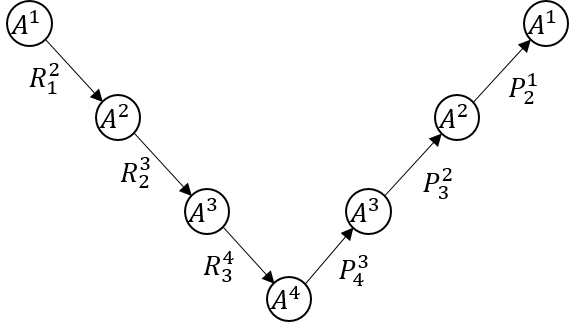
\includegraphics[width=0.5\textwidth]{chap04/figs/cicloV.png} \label{fig:ciclov}}
\qquad
\subfigure[Ciclo W ]{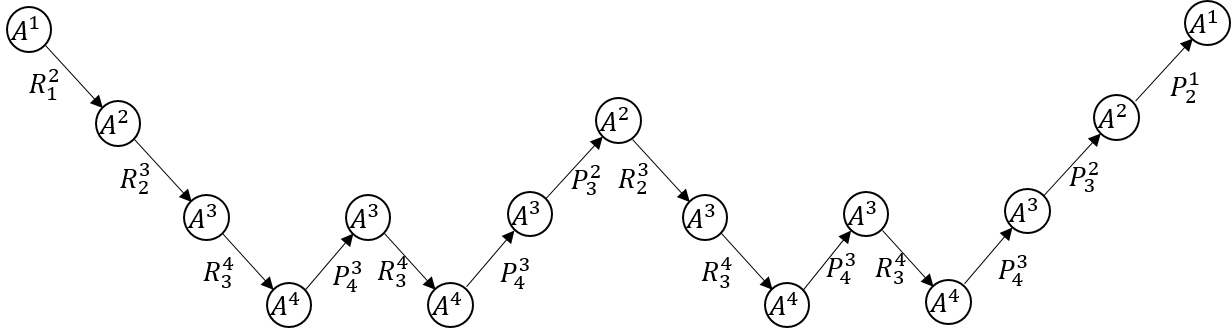
\includegraphics[width=0.8\textwidth]{chap04/figs/cicloW.png} \label{fig:ciclow}}
\caption{Aplicação de um ciclo V e W com quatro níveis. Os círculos $A_1$, $A_2$, $A_3$ representam relaxações com esses operadores, enquanto o círculo relacionado a $A_4$ representa a solução direta de um sistema linear. }\label{fig:exemplomultigrid}
\end{figure}




\begin{algorithm}[H]
\caption{Ciclo-V($A_1$, $A_2$, $x_0$, $b$)}
\label{alg:ciclomg2niveis}
\Inicio{

$x_0 \leftarrow \text{relaxação}(A_1, x_0, b)$, $\upsilon_1$ vezes

$r \leftarrow b - A_1 x_0$

$r \leftarrow R^2_1 r$

$\delta_2 \leftarrow A_2^{-1} r$

$\delta_1 \leftarrow P^1_2 \delta_2$

$x_0 \leftarrow x_0 + \delta_1$

$x_0 \leftarrow \text{relaxação}(A_1, x_0, b)$, $\upsilon_2$ vezes
}

\end{algorithm}

\vspace{1cm}
\begin{algorithm}[H]
\caption{Ciclo-$\mu$($i$, $\mu$, $x$, $b$, $A_1$, $A_2$, ...) (Adaptado de \cite{multigridtutorial})}
\label{alg:ciclomu}
\Inicio{

$\text{relaxação}(A_i, x)$, $\upsilon_1$ vezes

$b_i \leftarrow R^{i+1}_i (b - A_i x)$


\Se{i + 1 é o nível mais grosso}{
    $x_{i+1} \leftarrow A_i^{-1} f$
}
\Senao{
    $x_{i+1} \leftarrow \mathbf{0}$

    $x_{i+1} \leftarrow x_{i+1} $ Ciclo-$\mu$($i+1$, $\mu$, $x_i$, $b_i$, $A_1$, $A_2$, ...), $\mu$ vezes
}

$x \leftarrow  x + P^i_{i+1} x_{i+1}$

$\text{relaxação}(A_i, x)$, $\upsilon_2$ vezes
}

\end{algorithm}
\vspace{1cm}


\subsubsection{Relaxações}


Em relação as relaxações utilizadas pelo método multigrid, duas bastante utilizadas são a Jacobi e o Gauss-Seidel. Elas tem como intuito remover os erros de alta frequência em cada um dos níveis multigrid. Em particular, a relaxação de Gauss-Seidel simétrica foi utilizada na comparação do Capítulo \ref{ch:resultados} e é mostrada no Algoritmo \ref{alg:gauss_seidel} que foi retirado do código do Pyamg. É importante notar que, nesse caso, a quantidade de operações feitas é proporcional a duas vezes o número de não zeros da matriz , pois, a relaxação é realizada começando de i=1 e depois voltando de i=n. Uma outra maneira de implementar o Gauss-Seidel é a apresentada em \cite{solverlinear} onde as iterações são definidas pela recorrência: $x^{k+1/2}=x^k+(L+D)^{-1}r^k$ e $x^{k+1}=x^{k+1/2}+(D+U)^{-1}r^{k+1/2}$.


\vspace{1cm}

\begin{algorithm}[H]
\caption{Gauss-Seidel-Simétrico(A, x, b)}
\label{alg:gauss_seidel}
\Inicio{

$n \leftarrow \text{Tamanho de } A$

\Para{ $i \in 1,2,3,\cdots,n$}{
    \Para{$j \in 1,2,3,\cdots,n$}{
        $x(i) \leftarrow b(i)$
        
        \Se{$j \ne i$}{
            $x(i) \leftarrow x(i) - A(i,j) \times x(j)$
        }
    }
    $x(i) \leftarrow x(i)/A(i,i)$
}

\Para{ $i \in n,n-1,n-2,\cdots,1$}{
    \Para{$j \in 1,2,3,\cdots,n$}{
        $x(i) \leftarrow b(i)$
        
        \Se{$j \ne i$}{
            $x(i) \leftarrow x(i) - A(i,j) \times x(j)$
        }
    }
    $x(i) \leftarrow x(i)/A(i,i)$
}
}
\end{algorithm}

\vspace{1cm}


\subsubsection{Complexidade do Grid}
 
O PyAmg possui um método para os seus solver para cálculo da  Complexidade do Grid, esse valor tenta representar o quão mais custoso é a utilização de um determinado solver multigrid em relação ao operador original. A definição é mostrada em \eqref{eq:complexidadegrid}. Como pode-se ver, ele conta quantos não zeros o somatório de todos os níveis possui a mais que o nível fino. Assim, por exemplo, considerando $\upsilon_1=1$ e $\upsilon_2=1$ cada nível irá realizar duas relaxações, com exceção do nível mais grosso, tornando o  custo de um ciclo aproximadamente $2\times\text{Complexidade Grid}$. 

\begin{equation}\label{eq:complexidadegrid}
    \text{Complexidade Grid} = \frac{\sum_{i=1}^n \text{nnz}(A_i)}{\text{nnz}(A_1)}
\end{equation}

Para saber o custo de um ciclo W se torna mais complicado devido a recursão associada a esse tipo de ciclo. No caso do ciclo apresentado na Figura \ref{fig:ciclow}, são feitas duas relaxações com $A_1$ e quatro com $A_2$ (o vértice $A_2$ do meio em que chega e sai uma seta acontecem duas relaxações) e oito relaxações com $A_3$. O PyAmg também tem um método que cálcula a complexidade do ciclo através de recursão e foi utilizado para as comparações apresentadas no Capítulo \ref{ch:implementacao}. 

%Primeiramente, é possível encontrar o ponto de mínimo ao de caminhar a partir ponto inicial $x_0$ e uma direção $d_0$. Dessa forma, sendo $x_1 = x_0 + \alpha d_0$ para encontrar o ponto que minimiza o $f(x_1)$ deve-se ter $\frac{d f(x_1)}{d\alpha} = 0$.

%\begin{equation}
%    \frac{df(x_1)}{d \alpha} =  \nabla f(x_1)^T d_0 = 0
%\end{equation}

%Pela equação \ref{eq:gradf}, $\nabla f(x_1) = -r_1 $ então:


% \begin{align}
%      r_1^T r_0                         & =  0 \\
%      r_0^T r_1                         & =  0 \\
%      r_0^T (b - Ax_1)                  & =  0 \\
%      r_0^T (b - A(x_0 - \alpha d_0))   & =  0 \\
%      r_0^T (b - Ax_0  - \alpha A d_0)  & =  0 \\
%      r_0^T (r_0 - \alpha A d_0)        & =  0 \\
%      r_0^T r_0 - \alpha  r_0^T A d_0   & =  0 \\
%      \alpha  r_0^T A d_0               & =  r_0^T r_0 \\
%      \alpha                            & =  \frac{r_0^T r_0}{r_0^T Ad_0}
% \end{align}

% O método dos gradientes conjugados em andar em direções conjugadas a cada passo de tempo minimizando $f(x)$ naquela direção. A direção inicial escolhida é

\section{Fatoração LU} \label{sec:fatoracaolu}

Outra parte importante para esse trabalho é a solução direta de sistemas, em particular por conta dos sistemas que serão resolvidos nos espaços grossos e também para cálculo das funções de base que serão apresentados no Capítulo \ref{ch:multiescala}. Esses sistemas tem um número reduzido de variáveis em comparação com os sistemas associados com o grid fino e, portanto, pode-se pensar na utilização de solvers diretos.

A fatoração LU consiste em transformar a matriz A em o produto de outras duas $\mathbf{A}=\mathbf{L}\mathbf{U}$: $\mathbf{L}$ triangular inferior e $\mathbf{U}$ triangular superior. Assim, o sistema fica da forma $\mathbf{L} \mathbf{U} \mathbf{x} = \mathbf{b}$ e a solução é realizada através da solução de dois sistemas triangulares $\mathbf{L}\mathbf{y} = \mathbf{b}$ e $\mathbf{U}\mathbf{x} = \mathbf{y}$. O cálculo dos fatores LU pode ser feita utilizando uma eliminação gaussiana e pode ser encontrado em \citet{heath1997scientific}. Uma vantagem desse método é que se for necessário resolver sistemas para diferentes lados direito $\mathbf{b}$ a fatoração pode ser reutilizada e não precisa ser calculada novamente. Para matrizes simétricas positivas definidas, existe a fatoração de Cholesky, similar a fatoração LU, onde $\mathbf{A} = \mathbf{C}^T \mathbf{C}$, com $C$ triangular superior.


\subsubsection{Precondicionador ILU}

Os precondicionadores baseados em fatoração incompletas (ILU) apresentados em \citet{ilupaper} calculam uma aproximação para a fatoração LU da matriz. A aproximação é realizada desconsiderando algumas entradas das matrizes $\mathbf{L}$ e $\mathbf{U}$. Um parâmetro do método é o nível do ILU que controla a quantidade de entradas que a fatoração incompleta possui; quando o nível é  zero, a fatoração possui não zeros nas mesmas posições em que a matriz $\mathbf{A}$ possui entradas não-nulas. Há várias outras alternativas baseadas em aproximações da fatoração LU, ver \cite{solverlinear}.


  \chapter{Operadores Multiescala}\label{ch:multiescala}
  
Nesse capítulo, será apresentada a construção do operador grosso Multiescala. A construção desse tipo de operador tem diversas aplicações para a solução dos sistemas lineares apresentados no Capítulo \ref{ch:discretizacao}. Ele consiste basicamente em construir um operador grosso através do cálculo de funções de base em um grid gerado pelo acoplamento de elementos do grid fino. Pode ser utilizado como pré-condicionador \cite{casteletto}, como solver multinível semelhante aos solver multigrid ou ainda como aproximação para a solução original do problema. Os métodos multiescala tem sido aplicados com sucesso para problemas elípticos que é o caso do problema da elasticidade linear apresentado aqui. As vantagens do método discutido em \cite{thomashou} são que as funções de base multiescala tentam se adaptar às propriedades locais do operador, de forma que o operador grosso as conserve. As funções de base podem ser construídas através da solução de problemas independentes e, portanto, em paralelo.

O primeiro passo para a construção do operador multiescala é gerar um novo grid com menos elementos que o grid original do problema (grid fino), mas que ainda represente o mesmo domínio $\Omega$. Esse novo grid será chamado de grid grosso e as variáveis relacionadas com ele serão assinadas com o sobrescrito $H$. 
Assim grid grosso possui um conjunto $\tau_H$ de elementos onde cada elemento será uma aglomeração de elementos do grid fino. Por exemplo, a Figura \ref{fig:gridgrosso} apresenta um grid grosso $3\times 3$ construído a partir de um grid fino $7\times 7$. É importante perceber que não existe a necessidade de aglomerar a mesma quantidade de elementos do grid fino para se gerar um elemento do grid grosso, já que existem elementos formados por 9, 6 ou 4 elementos do grid fino. OS quadrados azuis destacam os nós que pertencem ao grid grosso e ao grid fino simultaneamente.

\begin{figure}[!htbp]
\centering
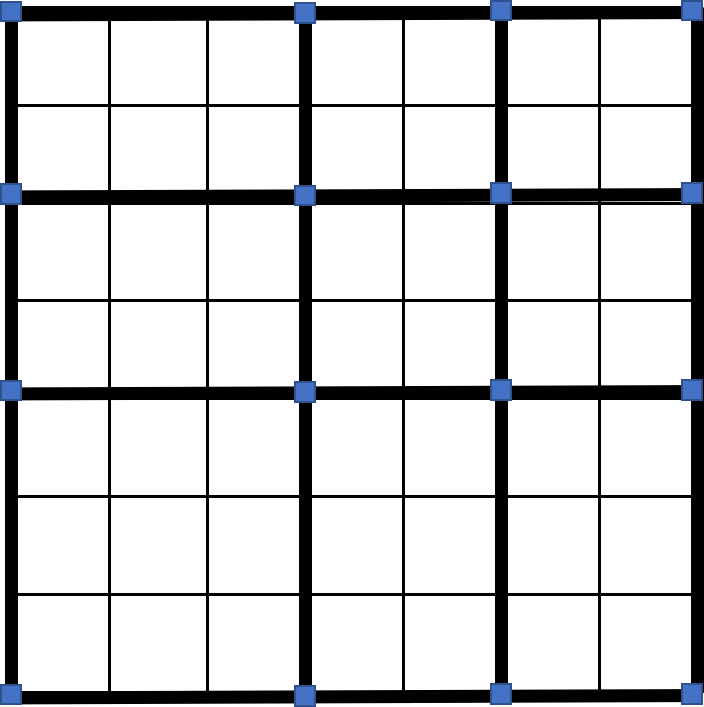
\includegraphics[width=6cm]{chap06/figs/grosso.png}
\caption{Exemplo de grid fino $7\time 7$ e um grid grosso $3\times 3$. O elemento inferior esquerdo é composto por 9 elementos do grid fino enquanto o elemento superior direito é composto com 4 elementos do grid fino.}
\label{fig:gridgrosso}

\end{figure}


No Capítulo \ref{ch:discretizacao} foi apresentada a discretização  para o problema de elasticidade linear através do método dos elementos finitos, com notação baseada em \cite{mbuck}. Naquele capítulo, a função desejada foi aproximada em um espaço $V^h$ formado por funções de base chapéu, no domínio $\Omega$ do problema. Agora vamos encontrar a solução do problema em um espaço grosso $V^{MS}$, tal que $V^{MS} \subset V^h$. 



Para estabelecer o espaço $V^{MS}$, precisamos definir as suas funções de base geradoras. 
Novamente, para distinguir o nó pertencente ao grid grosso dos seus graus de liberdade, o seguinte conjunto com graus de liberdade é criado:


\begin{equation}\label{eq:dheq}
    D^H = \{ p^{(m)} \in D^h : x^p \in \Sigma_H, m=1,2\}.
\end{equation}

\suge{acho que vc deveria esclarecer aqui cada um dos elementos da equação \eqref{eq:dheq}, mesmo que já tenha feito isso em algum capítulo anterior}

\section{Cálculo do NNZ do operador de prolongamento}\label{sec:complexProlong}

Em um método multiescala, além da construção de um operador grosso,  precisa-se mover os vetores entre os espaços fino e grosso  Essas movimentações são realizadas através de multiplicação por operadores especiais, $P$ e $P^T$. Essa seção descreve a complexidade destas operações.

As dimensões do operador de prolongamento dependem dos graus de liberdade do operador fino e do  grosso, valendo $\freedomfine \times \freedomcoarse$. Conforme visto no Capítulo \ref{ch:sistemas}, a multiplicação de uma matriz esparsa por um vetor é da ordem do número de elementos  não nulos da matriz, assim, apesar de um maior engrossamento do grid reduzir o valor de $n_u^H$,  não necessariamente ocorre  uma redução de elementos não nulos de $P$. \suge{Talvez uma forma simples de motivar esta ideia, seja dizer que todos os elementos a matriz $A$ tem que ser multiplicados por algum elemento da matriz de restrição, não podendo ficar nenhum de fora, sendo assim, mesmo que ser reduza o número de linhas do operador de restrição, a quantidade de elementos não nulos não pode ser alterada. O que ocorre é que cada linha do operador de restrição, ou coluna do de extensão, fica mais densa quando se diminui a dimensão do espaço grosso}

Considerando um grid fino com $\numelementsxfine \times \numelementsyfine$, um grid grosso onde cada elemento tem dimensões $q_x \times q_y$ \suge{neste caso você está considerando que os elementos grossos são formados sempre pelo mesmo número de elementos, talvez seja o caso de dizer que você vai fazer isso mais lá em cima, apesar de isso não ser necessário} e, ainda, que mesmo os nós de fronteira com condição de contorno de Dirichlet não são removidos da matriz de rigidez, então a quantidade de não zeros do operador de prolongamento ($nnz_p$) pode ser calculada contando os nós de três conjuntos:  nós interiores, nós no vértice e os nós na aresta.  A Figura \ref{fig:gridCompleto} mostra cada um desse tipo de nós (em vermelho nó no vértice, em azul nó na aresta e em preto nó interior).


\begin{figure}[h]
\center
\subfigure[  ]{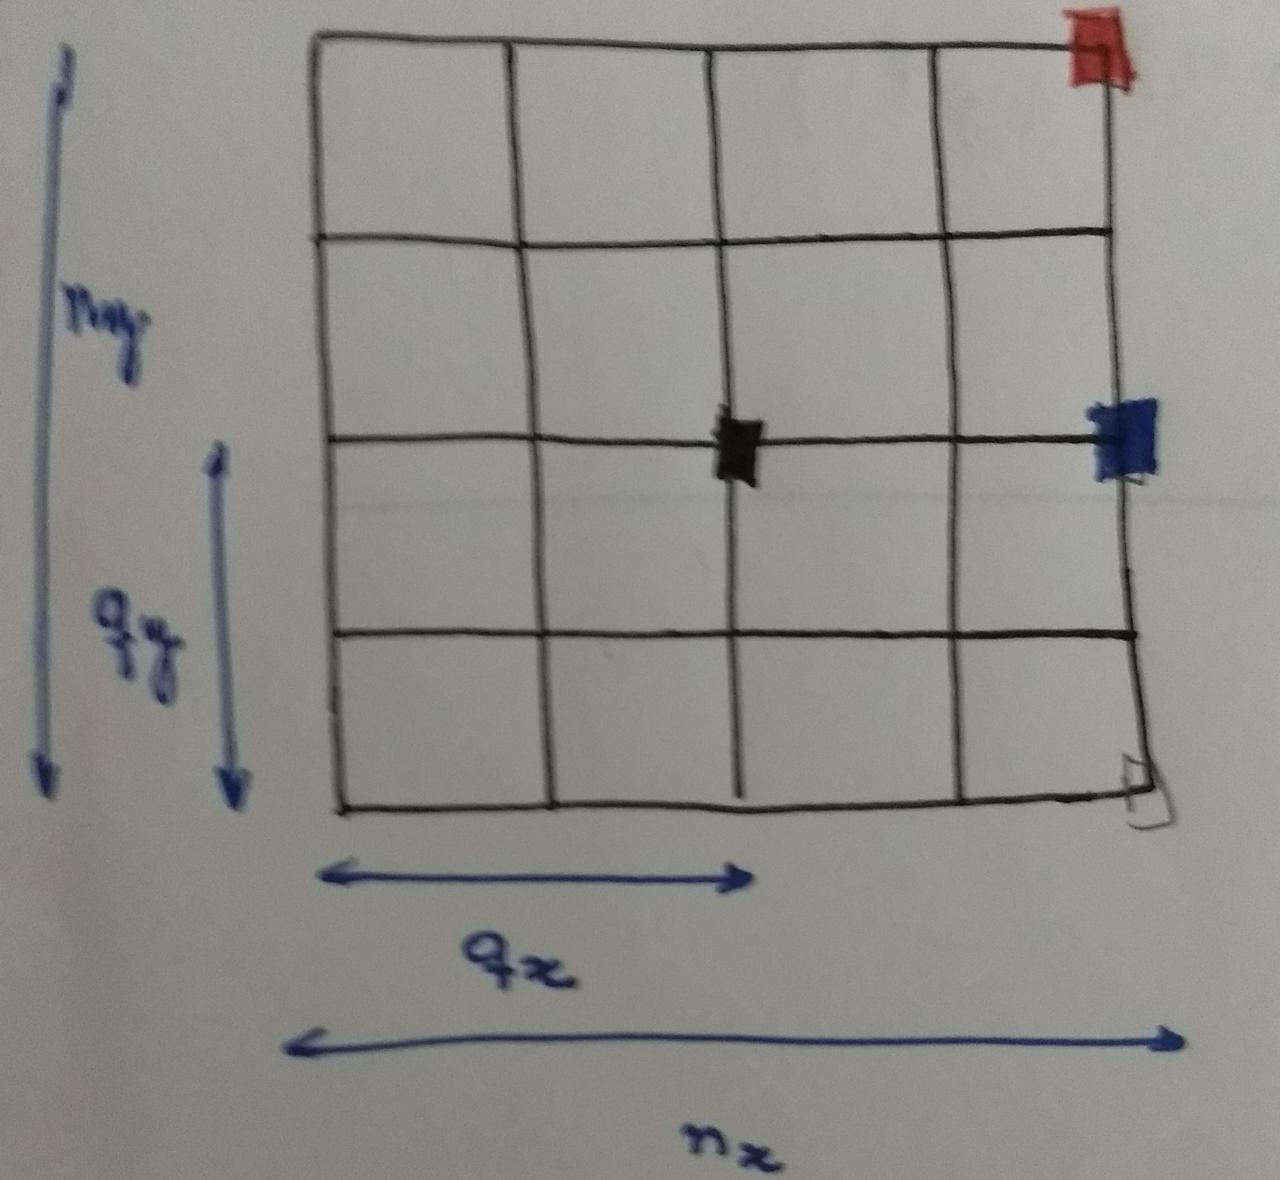
\includegraphics[width=0.45\textwidth]{chap06/figs/gridCompleto.jpeg}\label{fig:gridCompleto}}
\qquad
\subfigure[ ]{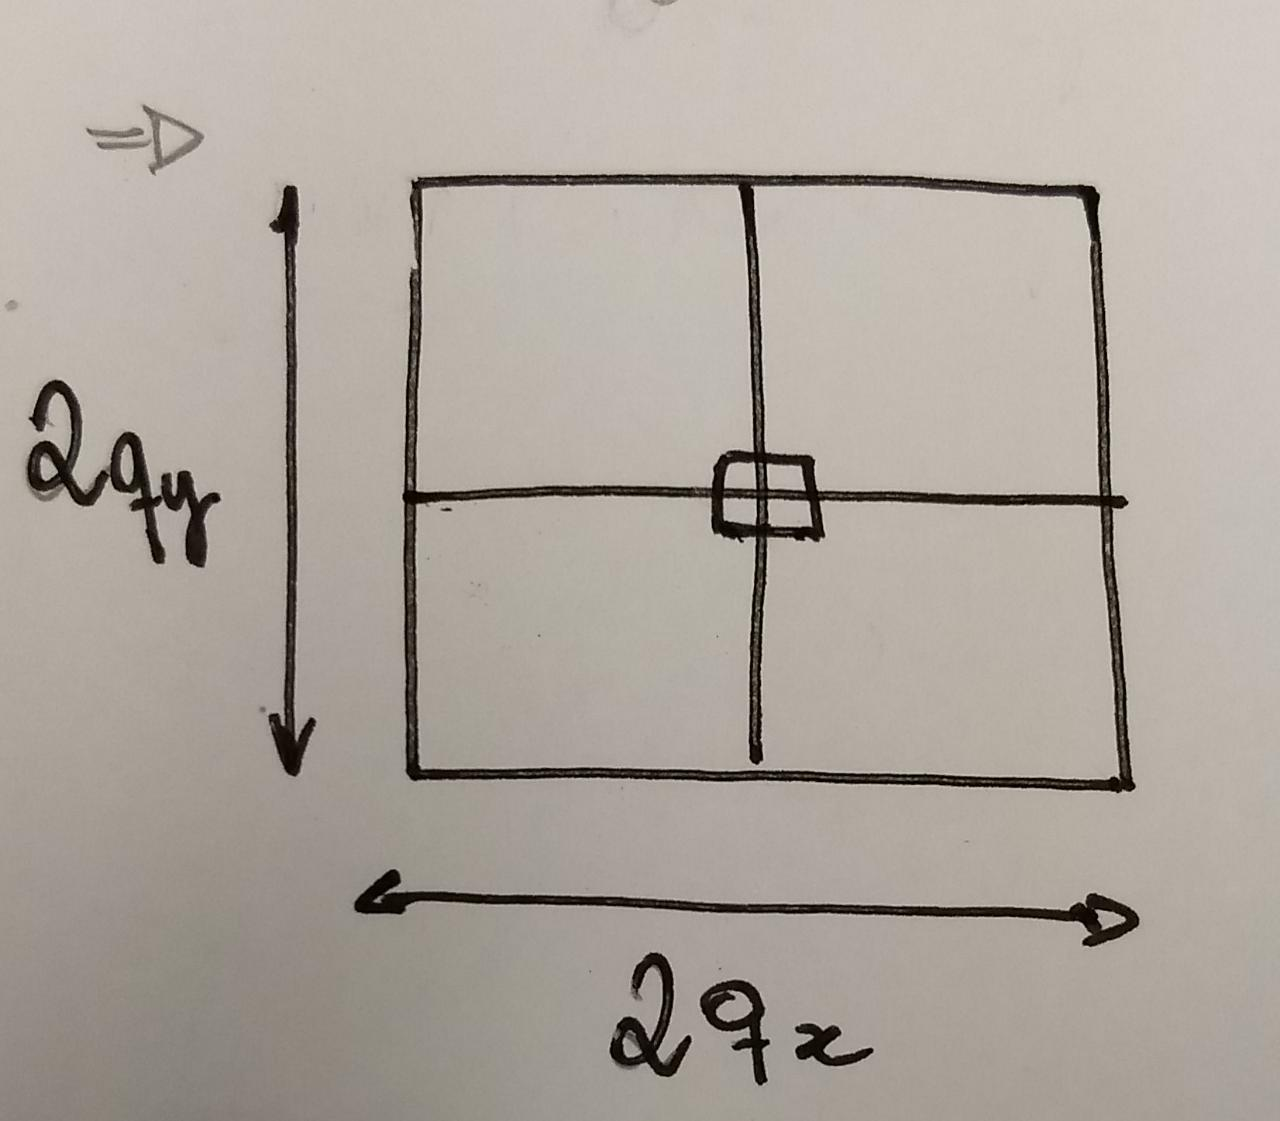
\includegraphics[width=0.45\textwidth]{chap06/figs/noInterior.jpeg}\label{fig:noInterior}}
\subfigure[ ]{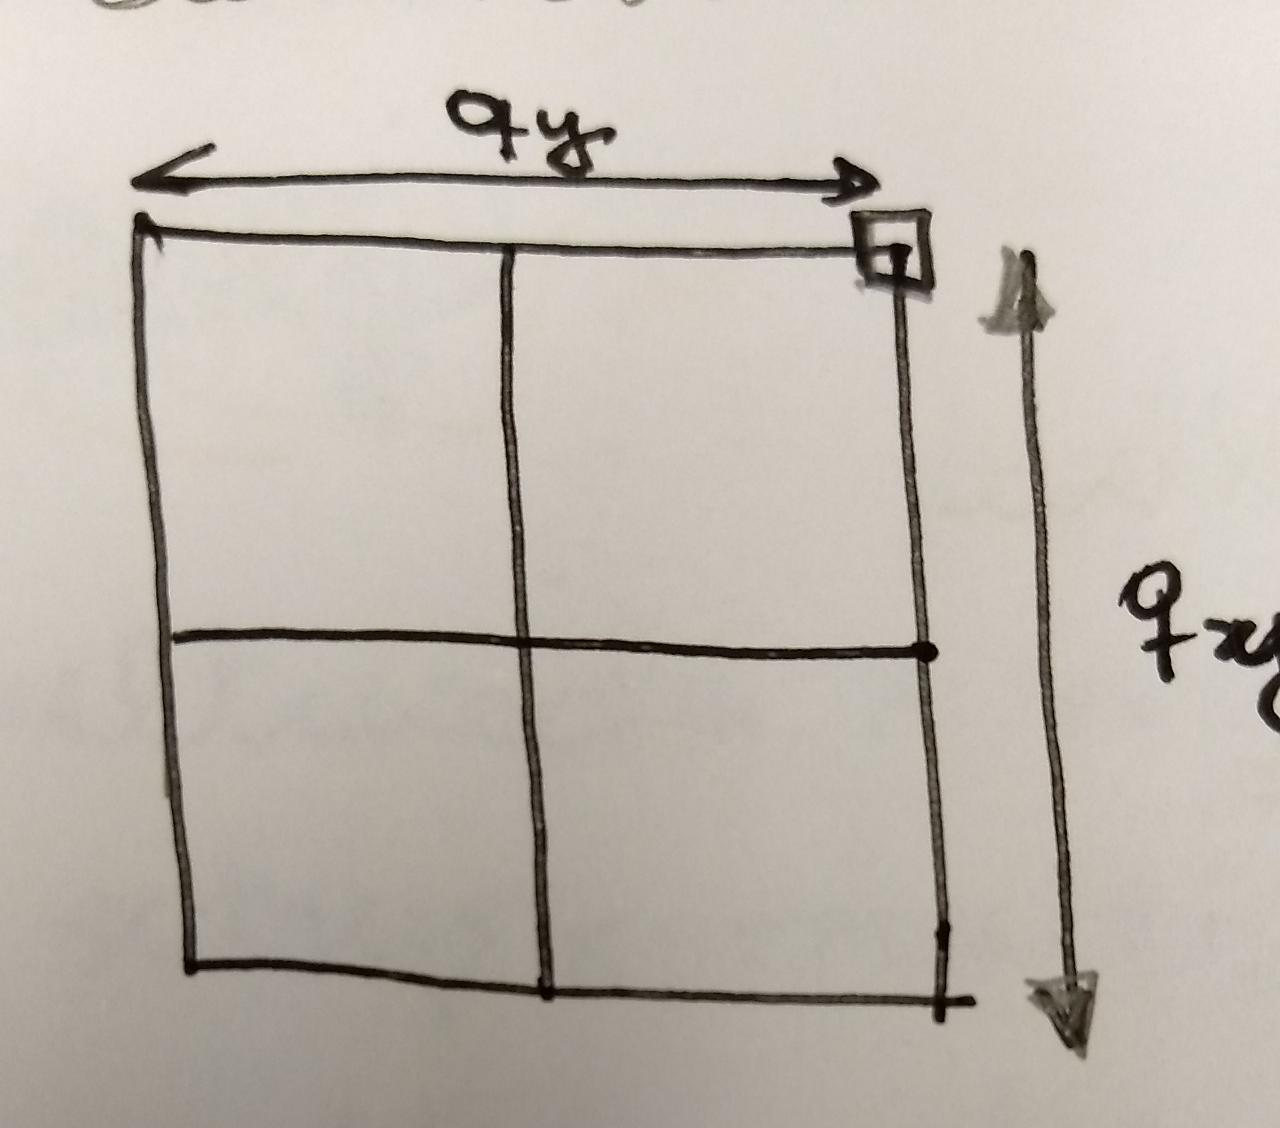
\includegraphics[width=0.45\textwidth]{chap06/figs/noVertice.jpeg}\label{fig:noVertice}}
\subfigure[ ]{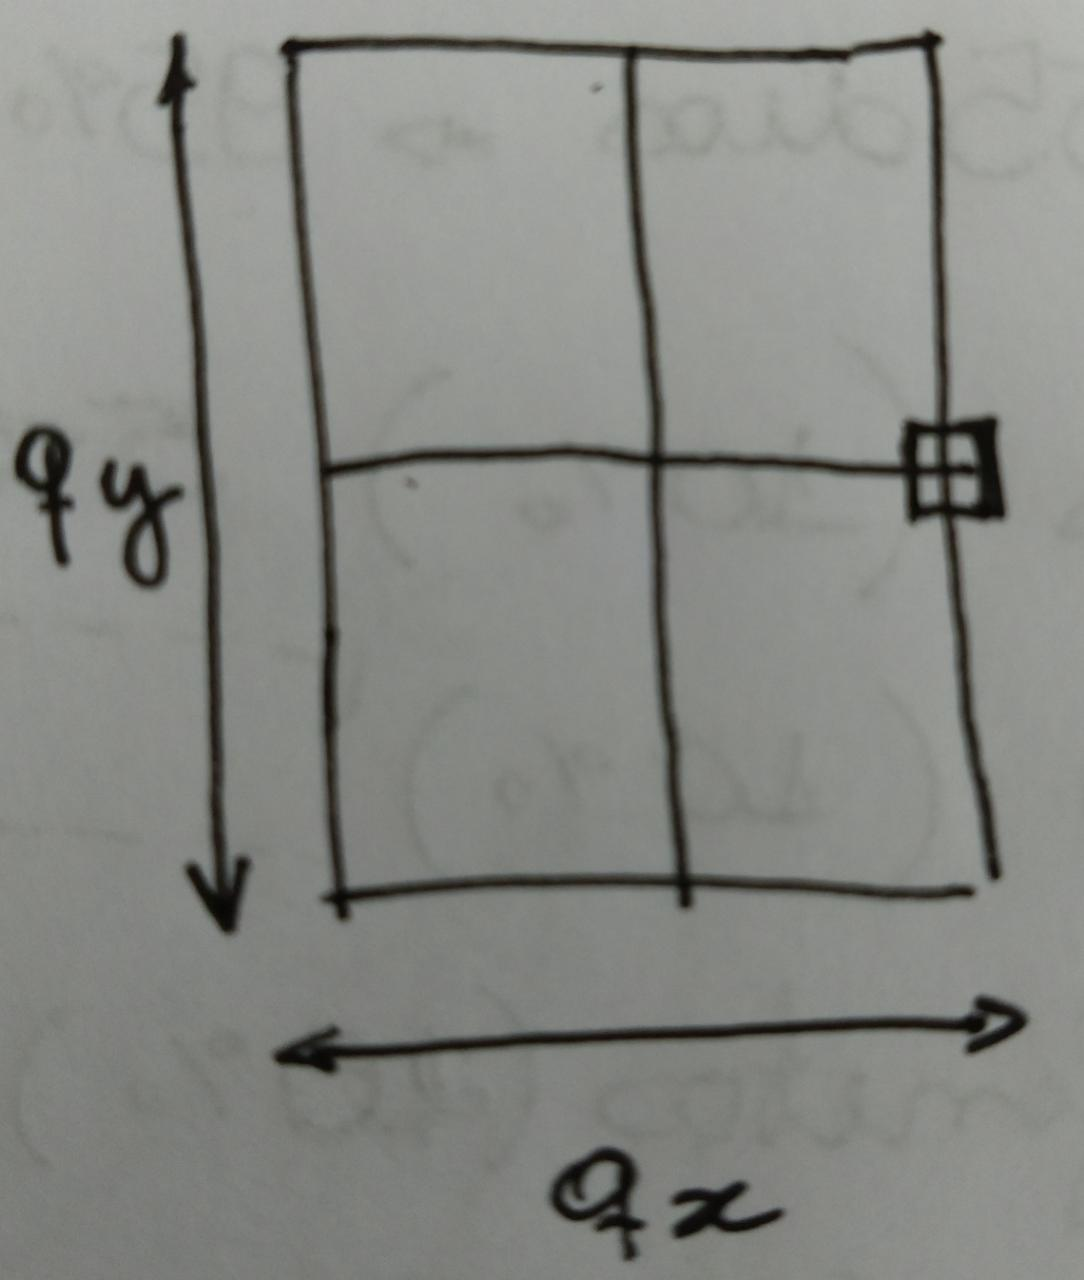
\includegraphics[width=0.45\textwidth]{chap06/figs/noAresta.jpeg}\label{fig:noAresta}}

\caption{Comparação da solução do grid fino com a solução do grid grosso.  }
\label{fig:verticesTypes}
\end{figure}

A quantidade de cada um desses nós na malha grossa é apresentado abaixo.

\begin{itemize}
    \item Nós interiores: $(\frac{n_x}{q_x} - 1) (\frac{n_y}{q_y} - 1)$
    \item Nós de aresta em $\Gamma_l$ e $\Gamma_r$: $2 ( \frac{n_y}{q_y} - 1)$
    \item Nós de aresta em $\Gamma_t$ e $\Gamma_b$: $2 ( \frac{n_x}{q_x} - 1)$
    \item Nós vértices: 4 
\end{itemize}


Cada nó tem duas funções de base associadas uma para cada grau de liberdade (x e y). Uma função de base de um vértice interior tem suporte \suge{como vc está definindo suporte? Em matemática, são os pontos do domínio onde a função é diferente de zero e, me parece, que não é isso que vc está dizendo. Acho que vc está falando de que haverá esse número de funções de base que estarão relacionadas a um nó interior. Ou seja a função definida no próprio nó e as funções definidas nos nós vizinhos, interiores ou não. Essa relação dá o número de elementos não nulos da linha desse nó interior} em $(2q_x+1)(2q_y+1)$ outros nós, como mostra a \ref{fig:noInterior}. Além disso, ela afeta os dois graus de liberdade de cada um desses nós, então cada um deles contribui com $4(2q_x+1)(2q_y+1)$ \perg{por que 4} não zeros para o prolongamento (uma implementação mais cuidadosa do método pode economizar as bordas do suporte pois as funções se anulam). De maneira análoga, os nós vértices contribuem com $ 4 (q_x+1)(q_y+1)$, os nós aresta em $\Gamma_t$ e $\Gamma_b$ contribuem com $ 4 (2q_x+1)(q_y+1) $ e, finalmente, os nós arestas  $\Gamma_l$ e $\Gamma_r$ e contribuem com $ 4(q_x+1)(2q_y+1) $. Assim, para encontrar a quantidade total de não zeros do operador de prolongamento, basta multiplicar as quantidades de cada um dos nós pela duas contribuições conforme a   \eqref{eq:nnzRaw}. 


\begin{equation} \label{eq:nnzRaw}
\begin{aligned}
    nnz_P = & 4(2q_x+1)(2q_y+1)  (\frac{n_x}{q_x} - 1) (\frac{n_y}{q_y} - 1)   \\ 
            & + 4 (q_x+1)(2q_y+1)  2 ( \frac{n_y}{q_y} - 1) +  4 (2q_x+1)(q_y+1)  2 (\frac{n_x}{q_x} - 1) \\
            & +  4(q_x+1)(q_y+1) 4 
\end{aligned}
\end{equation}

Que pode ser modificada para a \eqref{eq:nnzRaw2},

\begin{equation} \label{eq:nnzRaw2}
\begin{aligned}
    nnz_P = &   4 (2+\frac{1}{q_x})(2 + \frac{1}{q_y})  (n_x - q_x) (n_y - q_y) \\ 
            & + 8 (q_x+1)(2 + \frac{1}{q_y})  (n_y - q_y) \\
            & + 8 (2+\frac{1}{q_x})(q_y+1) (n_x - q_x) \\
            & + 16 (q_x+1)(q_y+1)  
\end{aligned}
\end{equation}

Assim, se $q_x$ e $q_y$ são de ordem $O(1)$ o primeiro termo da soma é da ordem de $O(n_x \times n_y)$. Caso $q_x$ e $q_y$ sejam de ordem $O(n_x)$ e $O(n_y)$, então o último termo da soma é da ordem $O(n_x \times n_y )$. \suge{não vejo muito sentido em $q_x$ ser $O(1)$, pois $q_x$ e $n_x$ vão sempre ter uma relação direta e, neste caso, o conceito de ordem esconde a constante de proporcionalidade e não ajuda a definir bem a complexidade do problema. $q_x$ e $n_x$ não teriam relação caso um fosse fixado e outro alterado, que é a situação mostrada na Figura \ref{fig:nnzGrafico}}
Se $q_x$ é $O(n_x)$ e $q_y$ é $O(1)$ então o segundo termo é de ordem $O(n_x \times n_y)$, analogamente para o caso contrário.
De toda forma, a quantidade de não zeros do prolongamento é da ordem do tamanho do grid $n_x \times n_y$ que é um fato importante, pois a multiplicação pelo prolongamento faz parte do processo de utilização do pré-condicionador multiescala e esse preço sempre terá que ser pago.\suge{tudo bem isso, é verdade, pois o operador de prolongamento tem $n_x \times n_y$ linhas, mas esse fato deve ser ponderado pelo número de colunas do operador} O valor limite também dos não zeros é representado pelo último termo da soma $16(q_x+1)(q_y+1)$. \suge{acho que vale a pena provar essa afirmação e não deixá-la apenas visual}

Um gráfico representando    \eqref{eq:nnzRaw2} é mostrado na Figura \ref{fig:nnzGrafico}, no eixo y é apresentado $nnz_P$ enquanto no eixo x é apresentado o engrossamento da malha que tem a mesma proporção em x e y ($q_x  = q_y$) para um grid de $1024 \times 1024$. Pelo gráfico é possível ver que o $nnz_P$ tende já em um engrossamento $16 \times 16$.


\begin{figure}[!htbp]
\centering
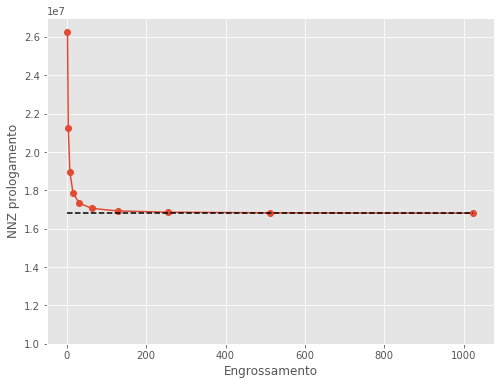
\includegraphics[width=8cm]{chap06/figs/nnzProlongamento.png}
\caption{Quantidade de não zeros do prolongamento $nnz_P$  em função do engrossamento da malha. A linha pontilhada mostra o valor de $16(n_x+1)(n_y+1)$.}
\label{fig:nnzGrafico}
\end{figure}


  \chapter{Implementação Computacional}\label{ch:implementacao}

  \chapter{Experimentos Numéricos}
  Nesse capítulo, serão apresentados os resultados obtidos utilizando o método multiescala para solução dos sistemas lineares decorrentes do operador apresentado no Capítulo \ref{ch:modelagem}. Os resultados são apresentados na seguinte ordem: resultados em casos que a solução analítica é conhecida,
comparação entre pré-condicionador aditivo e multiplicativo, comparações do pré-condicionador multiescala como e pré-condicionador multigrid e estudo do número de iterações do solver linear com variação da tolerância do solver grosso.



\section{Soluções Analíticas}

Inicialmente, é necessário atestar que o código de elementos finitos está resolvendo corretamente o operador descrito na Equação \ref{eq:edp_geomec}. 
Para isso, foi montado teste semelhante ao mostrado em \cite{irina}, teste consiste em encontrar solução para o problema que possui solução analítica de acordo com a equação mostrada em \ref{eq:irinasol} 
em um domínio $L \times W$.


\begin{equation} \label{eq:irinasol}
  \begin{aligned}
  u_x = 10^{-5} sen(\frac{\pi x}{L}) sen(\frac{\pi y}{W})  \\
  u_y = 10^{-5} sen(\frac{\pi (L-x)}{L}) sen(\frac{\pi x}{W})
  \end{aligned}
\end{equation}

Dada essa solução, é possível calcular o operador do lado direito aplicando o operador e obtendo a função $f: R^2 \rightarrow R^2$ apresentada em \ref{eq:irinald}. Dessa forma, as equações que representam o problema resolvido são apresentadas em \ref{eq:irinaproblem}, as condições de contorno nulas foram definidas como zero, pois é justamente o valor 

\begin{equation} \label{eq:irinald}
f(x, y) = 
\left[\begin{matrix}\frac{E \left(- 2 v + \pi^{2} y \left(v - 1\right) \left(y - 2\right) + 1\right) \sin{\left (\pi x \right )}}{\left(v + 1\right) \left(2 v - 1\right)} \\ \frac{\pi E \left(y - 1\right) \cos{\left (\pi x \right )}}{\left(v + 1\right) \left(2 v - 1\right)}\end{matrix}\right]
\end{equation}


\begin{equation}\label{eq:irinaproblem}
    \begin{aligned}
        S^T C S u = f(x, y) \\
        u(x,y) = [0, 0]^T, \text{ em } \Gamma \\
        L = W = 10
    \end{aligned}
\end{equation}


O erro entre a solução calculada pelo método dos elementos finitos pode então ser comparada
com a solução analítica pode ser calculado conforme a equação \ref{eq:erroAnalitico}.

\begin{equation} \label{eq:erroAnalitico}
    \epsilon_{inf} =\frac{|u_{fem} - u_{ref}|}{|u_{ref}|}
\end{equation}

onde $u_{ref} = [u_x(x_0, y_0), u_y(x_1, y_1), ..., u_x(x_{n_n}, y_{n_n})]^T$ e $u_{fem}$ é a solucão obtida com o método dos elementos finitos. Esse erro é mostrado na \ref{fig:SecondOrderTest} onde no eixo x 
está plotado no eixo x o logaritmo do tamanho de cada elemento e no eixo y o logaritmo do erro analítico também mostra uma reta de coeficiente angular $2$ para comparação com um decaimento
quadrático do erro em função do tamanho de cada elemento da malha.


\begin{figure}[h]

\center
\subfigure[ ]{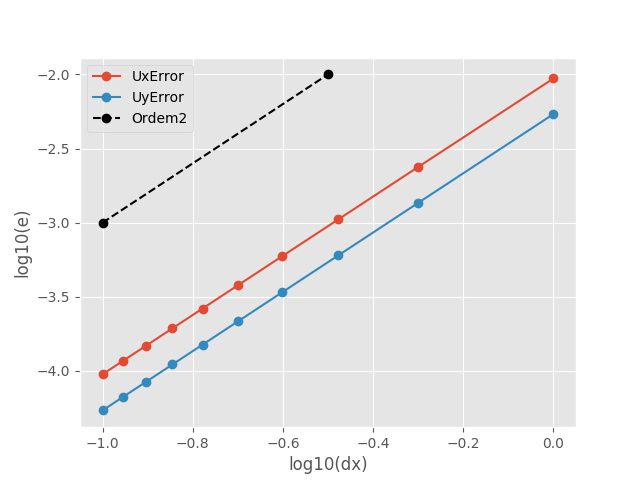
\includegraphics[width=0.45\textwidth]{chap08/figs/SecondErrorTest.png}\label{fig:SecondErrorTest}}
\qquad
\subfigure[ ]{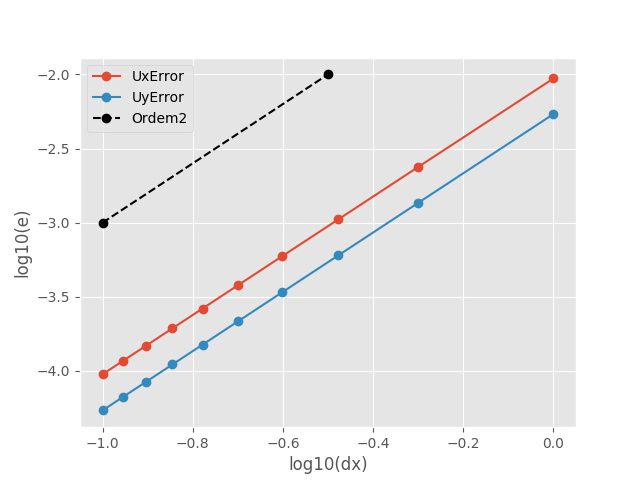
\includegraphics[width=0.45\textwidth]{chap08/figs/SecondErrorTest.png}\label{fig:subfig_b}}
\caption{Imagens lado a lado \ref{fig:SecondErrorTest}}
\end{figure}
    
    
Um segundo caso com resultado analítico é a condição de cisalhamento puro (Simple Shear). 
Nesse caso, o problema é definido na forma apresentada em \ref{eq:simpleshear}. A solução
é dada por $u(x,y) = [y, 0]^T$. Portanto, dado que o a solução é um polinômio do primeiro grau,
essa pode ser representada pelo espaço gerado pelas funções de base bilineares e, então,
os erros de truncamento nesse caso não existem ficando apenas com erros de arredondamento.

\begin{equation}\label{eq:simpleshear}
    \begin{aligned}
        S^T C S u = 0 \\
        u(x,y) = [10^{-6}, 0]^T, \text{ em } \{x, y \in \Gamma | y \neq 1\} \\
        u(x,y) = [10^{-6}y, 0]^T, \text{ em } \{x, y \in \Gamma | x = 0 \text{ ou } x = 1\} \\
        u(x,y) = [0, 0]^T, \text{ em } y=0
    \end{aligned}
\end{equation}

A variação do erro com o tamanho da malha é apresentado na figura \ref{fig:SecondErrorTestSimpleShear} e pode-se observar que nesse caso o maior erro relativo menor que $10^{-12}$ que é bem menor que do caso anterior por conta do erro de truncamento ser zero e também não decai com o tamanho da malha.

\begin{figure}[!htbp]
    \centering
    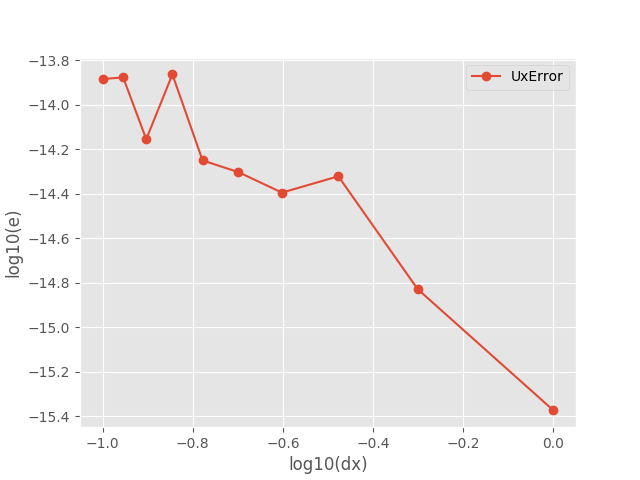
\includegraphics[width=7cm]{chap08/figs/SecondErrorTestSimpleShear.png}
    \caption{Comparação entre solução do grid fino e de diferentes grids grossos.}
    \label{fig:SecondErrorTestSimpleShear}
\end{figure}

Atestado o bom funcionamento do método dos elementos finitos para solução de problemas com a solução
analítica conhecida, será aplicado agora o método multiescala para verificar o seu correto funcionamento.

\section{Modelos de simulação utilizados}

Os resultados das próximas seções serão apresentados em utilizando os modelos apresentados na Tabela \ref{tab:descricaoModelos}. 
A tabela apresenta o tamanho dos grid dos modelos e se são baseados em casos reais ou não.


\begin{table}[]
    \caption{Tabela com os casos que serão apresentados os resultados. }\label{tab:descricaoModelos}
    \centering
    \begin{tabular}{ccccl}
    \cline{1-4}
    \multicolumn{1}{|c|}{\textbf{Nome}} & \multicolumn{1}{c|}{\textbf{Nx}} & \multicolumn{1}{c|}{\textbf{Ny}} & \multicolumn{1}{c|}{\textbf{Caso Real}} &  \\ \cline{1-4}
    \multicolumn{1}{|c|}{caso A}        & \multicolumn{1}{c|}{100}         & \multicolumn{1}{c|}{100}         & \multicolumn{1}{c|}{Não}                   &  \\ \cline{1-4}
    \multicolumn{1}{|c|}{caso B}        & \multicolumn{1}{c|}{320}         & \multicolumn{1}{c|}{320}         & \multicolumn{1}{c|}{Não}                   &  \\ \cline{1-4}
    \multicolumn{1}{|c|}{caso C}        & \multicolumn{1}{c|}{103}         & \multicolumn{1}{c|}{56}          & \multicolumn{1}{c|}{Não}                   &  \\ \cline{1-4}
    \multicolumn{1}{|c|}{caso D}        & \multicolumn{1}{c|}{244}         & \multicolumn{1}{c|}{71}          & \multicolumn{1}{c|}{Sim}                &  \\ \cline{1-4}
    \multicolumn{1}{|c|}{caso E}        & \multicolumn{1}{c|}{582}         & \multicolumn{1}{c|}{336}         & \multicolumn{1}{c|}{Sim}                &  \\ \cline{1-4}
    \multicolumn{1}{l}{}                & \multicolumn{1}{l}{}             & \multicolumn{1}{l}{}             & \multicolumn{1}{l}{}                    &  \\
    \multicolumn{1}{l}{}                & \multicolumn{1}{l}{}             & \multicolumn{1}{l}{}             & \multicolumn{1}{l}{}                    & 
    \end{tabular}
\end{table}


Os casos A e B são baseados nos casos sintéticos apresentados em \cite{casteletto} e \cite{irina}, nesses casos foram utilizados
uma compressibilidade vertical uniaxial $c_M$ desenvolvida em \cite{correlacaoE} apresentada na equação \ref{eq:correlacaoCm}

\begin{equation} \label{eq:correlacaoCm}
    c_M = 0.01241 |\sigma_y^\prime|^{-1.1342}
\end{equation}

onde $c_M$ e $\sigma_y^\prime$ são expressas em [bar$^{-1}$] e [bar] e  $\sigma_y^\prime$ representa a tensão vertical efetiva.
Considerando um gradiente de pressão de 0.1 bar/m e coeficiente de biot igual a um a tensão efetiva total pode ser calculada de acordo com \ref{eq:correlacaoTensao}.




\begin{equation} \label{eq:correlacaoTensao}
\sigma_y^\prime = \sigma_y + p = -0.12218|y| + 0.1 |y|
\end{equation}

E o módulo de Young pode ser calculado em função apenas da profundidade equação substituindo os valores de \ref{eq:correlacaoCm} e \ref{eq:correlacaoTensao} em \ref{eq:correlacaoYoung}.

\begin{equation} \label{eq:correlacaoYoung}
    E = \frac{(1-2\poisson)(1+\poisson)}{(1-\poisson)c_M}
\end{equation}

O grid utilizado é apresentado \ref{fig:gridBase10x10}, esse grid teve cada uma das células divididas em com 10 cortes verticais e 
10 cortes horizontais igualmente espaçados para gerar um o caso A e de forma análoga dividida em 32 cortes horizontais e 
32 cortes verticais para gerar o caso B.

\begin{figure}[!htbp]
    \centering
    
\includegraphics[height=4cm]{interrogacao.png}
    \caption{Grid base utilizado para construção dos casos A e B.}
    \label{fig:gridBase10x10}
\end{figure}

o caso C é um caso de reservatório sintético com grid de geometria mais próxima aos reservatórios reais, além disso, diferentemente dos casos A e B os valores
de poisson não são constantes ao longo do domínio. A figura \ref{fig:casoCgrid} apresenta o grid e os valores do módulo de Young e módulo de Poisson.
São apresentados também figuras dos casos D e E que tiveram as escalas omitidas por se tratarem de modelos de campos reais.


\begin{figure}[!htbp]
    \label{fig:casoCgrid}
    \centering
    
\includegraphics[height=4cm]{interrogacao.png}
    \caption{Propriedades (módulo de Young e coeficiente de poisson) para caso C }
\end{figure}


\begin{figure}[!htbp]
    \label{fig:casoDgrid}
    \centering
    
\includegraphics[height=4cm]{interrogacao.png}
    \caption{Propriedades (módulo de Young e coeficiente de poisson) para caso D }
\end{figure}

\begin{figure}[!htbp]
    \label{fig:casoEgrid}
    \centering
    
\includegraphics[height=4cm]{interrogacao.png}
    \caption{Propriedades (módulo de Young e coeficiente de poisson) para caso D }
    
\end{figure}


As condições de contorno utilizadas são representadas na figura \ref{fig:CondicoesContorno}. 

\begin{figure}[!htbp]
    \label{fig:CondicoesContorno}
    \centering
    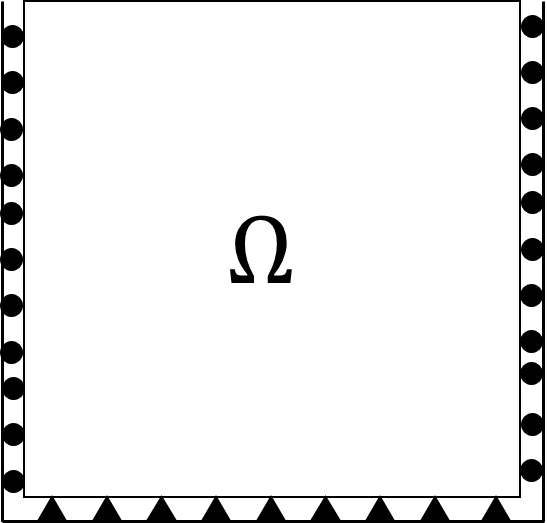
\includegraphics[height=4cm]{chap08/figs/CondicoesContorno.png}
    \caption{Esquema das condições de contorno das simulações. Borda inferior com deslocamentos nulos, bordas laterais com deslocamentos em y permitidos e borda superior livre.}
\end{figure}


\section{Método Multiescala como pré-condicionador}

\subsection{Comparação entre pré-condicionadores aditivos e multiplicativos}
O trabalho \cite{casteletto} apresenta a utilização do pré-condicionador multiescala ($M_{ms}$) em conjunto com o um pré-condicionador ($M_h$) no grid fino de forma multiplicativa. 
Essa combinação visa reduzir os erros de alta frequência através do $M_h$ enquanto os erros de baixa frequência são eliminados pelo pré-condicionador multiescala. 
O acoplamento multiplicativo tem a desvantagem de precisar de uma multiplicação matriz vetor além da aplicação dos pré-condicionadores
e, portanto, o número de iterações tem que ser reduzido o suficiente para compensar todas essas operações. Um alternativa é aplicação
dos pré-condicionadores de forma aditiva, pois, nesse caso, não é necessária a multiplicação matriz vetor adicional. Outra vantagem do operador
aditivo é que caso os dois pré-condicionadores sejam simétricos o pré-condicionador conjunto também é simétrico e pode ser utilizado juntamente
com o gradiente conjugado para a solução dos sistemas lineares.


Os testes as seguir mostram o número de iterações do Bicgstab utilizando pré-condicionadores multiplicativos e aditivos do caso A e caso B utilizados para comparação. É importante perceber que o pré-condicionador multiplicativo não necessariamente é simétrico e por isso o Gradiente Conjugado não tem garangia de convergia. Nesses testes o pré-condicionador $M_h$ utilizado foi o ILU(0).As tabelas \ref{table:precondcasoAcomp} e \ref{table:precondcasoBcomp} mostram a quantidade de iterações e os respectivos resíduos da solução do sistema linear.

É importante notar que a quantidade de iterações do dois métodos é bem próxima, em casos em que até o operador aditivo é mais eficiente que o multiplicativo. Assim, os testes que seguem utilizam como solver o gradiente conjugado. Dessa forma, os próximos
testes serão feito utilizando com o solver o Gradiente Conjugado.

\begin{table}[]
    \caption{Comparação de pré-condicionador aditivo contra multiplicativo para caso A utilizando como solver linear o método Bicgstab para diferentes níveis de engrossamento do nível grosso.}
    \label{table:precondcasoAcomp}
    \begin{tabular}{c|c|l|c|l|}

    \cline{2-5}
                                          & \multicolumn{4}{c|}{Pré-condicionador}                                                        \\ \cline{2-5} 
                                          & \multicolumn{2}{c|}{$\preconmult$}               & \multicolumn{2}{c|}{$\preconadd$}                \\ \hline
    \multicolumn{1}{|c|}{Elemento Grosso} & Iterações & \multicolumn{1}{c|}{Resíduo}      & Iterações & \multicolumn{1}{c|}{Resíduo}      \\ \hline
    \multicolumn{1}{|c|}{2x2}             & 7         & \multicolumn{1}{c|}{1.038308e-11} & 9         & \multicolumn{1}{c|}{8.186640e-12} \\ \hline
    \multicolumn{1}{|c|}{5x5}             & 16        & 1.720391e-11                      & 17        & 2.063517e-11                      \\ \hline
    \multicolumn{1}{|c|}{10x10}           & 25        & 1.872316e-11                      & 28        & 5.663356e-12                      \\ \hline
    \multicolumn{1}{|c|}{20x20}           & 38        & 1.643261e-11                      & 38        & 2.842643e-11                      \\ \hline
    \end{tabular}
\end{table}


\begin{table}[]
    \caption{Comparação de pré-condicionador aditivo contra multiplicativo para caso B utilizando como solver linear o método Bicgstab para diferentes níveis de engrossamento do nível grosso.}
    \label{table:precondcasoBcomp}
    \begin{tabular}{c|c|l|c|l|}
    \cline{2-5}
                                          & \multicolumn{4}{c|}{Pré-condicionador}                                                        \\ \cline{2-5} 
                                          & \multicolumn{2}{c|}{$\preconmult$}               & \multicolumn{2}{c|}{$\preconadd$}                \\ \hline
    \multicolumn{1}{|c|}{Elemento Grosso} & Iterações & \multicolumn{1}{c|}{Resíduo}      & Iterações & \multicolumn{1}{c|}{Resíduo}      \\ \hline
    \multicolumn{1}{|c|}{32x32}           & 86        & \multicolumn{1}{c|}{4.352864e-11} & 80        & \multicolumn{1}{c|}{4.187004e-11} \\ \hline
    \multicolumn{1}{|c|}{64x64}           & 126       & 4.645286e-11                      & 119       & 2.214093e-11                      \\ \hline
    \multicolumn{1}{|c|}{80x80}           & 133       & 4.939883e-11                      & 135       & 3.432757e-11                      \\ \hline
    \end{tabular}
\end{table}


\subsection{Comparação com Multigrid}

Nessa seção, são apresentadas comparações entre o método multiescala e o método multigrid. Para esse comparação foi utilizado o solver multigrid Pyamg, que é um solver multigrid  descrito e implementado em \cite{OlSc2018}. Dado a grande quantidade de parâmetros necessários para a configuração dos solver multigrid, como: a quantidade de níveis devem ser utilizados, quantidade de relaxações em cada nível, qual o tipo de relaxação será utilizada, dentre outras variáveis, foi utilizado o script solver\_diagnotics.py disponibilizado pela equipe do Pyamg no repositório ( https://github.com/pyamg/pyamg-examples ). Esse script testa diferentes configurações de solver multigrid para uma dada matriz e seleciona aquele mais eficiente para o problema proposto.

Os resultados para cada uma das matrizes mostrou um solver comum a todas as matrizes que possuía os seguintes parâmetros:

\begin{itemize}
    \item máximo de quinze níveis multigrid
    \item relaxação "Block Gauss Seidel Sweep" 
    \item ciclos V
    \item multigrid como pré-condicionador para o Gradiente Conjugado
\end{itemize}

A figura \ref{fig:reservatorio100x100_1} apresenta o tempo de solução do sistema utilizando o método multiescala e multigrid (Pyamg) como precondicionador para o gradiente conjugado para o caso A. São apresentados o resíduo ao longo das iterações, o tempo de execução do solver, a quantidade de iterações do solver linear e o tempo da iteração.

\begin{figure}[!htbp]
\centering
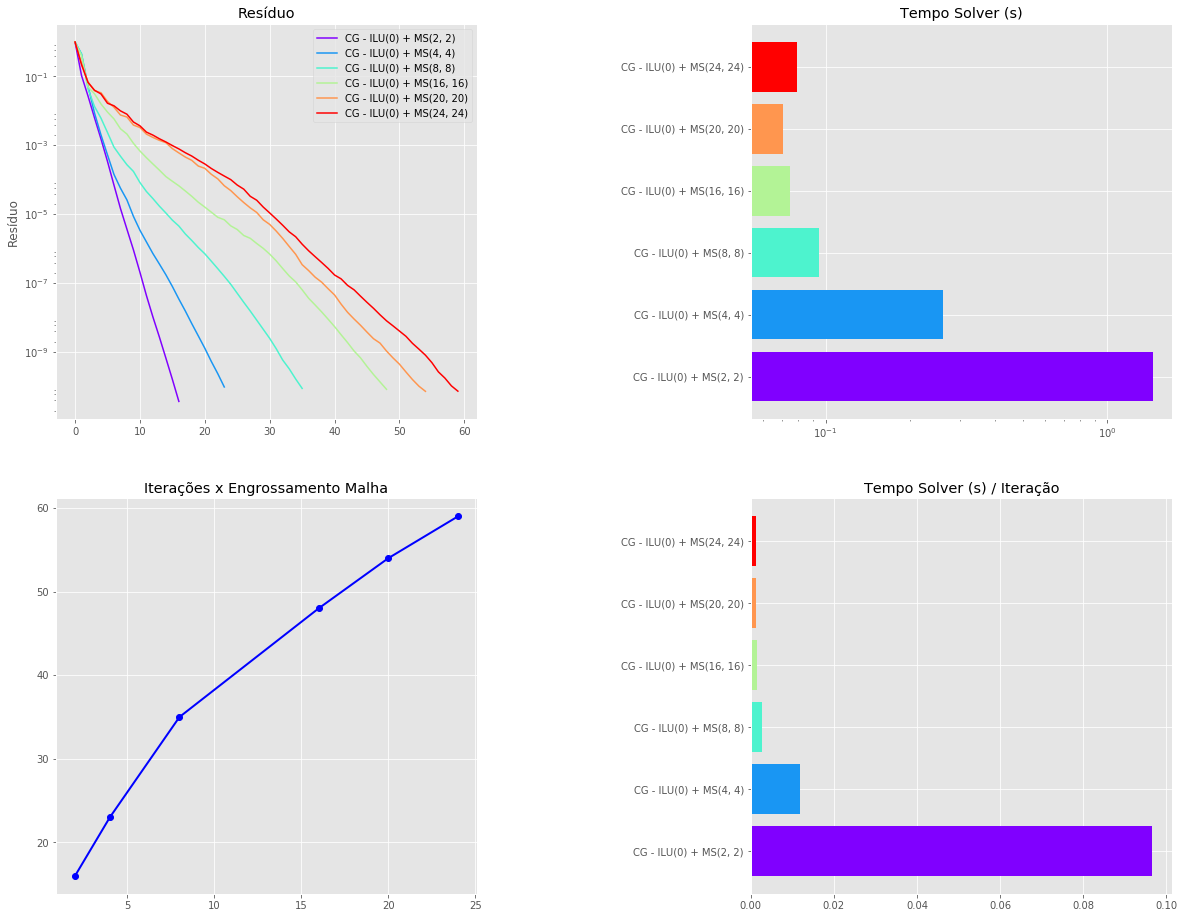
\includegraphics[width=\textwidth]{chap08/figs/reservatorio100x100_1.png}
\caption{Resultados para caso A. À esquerda Histórico do resíduo relativo ao longo das iterações. 
Ao centro, tempo do solver em segundos. À direita o tempo do solver por iteração. }
\label{fig:reservatorio100x100_1}
\end{figure}

Um primeiro ponto a se observar no gráfico da esquerda é o aumento do número de iterações a cada vez que se aumenta o fator de engrossamento da malha. Isso ocorre pois a solução do problema grosso se torna cada vez mais distante da solução da malha fina fazendo com que o pré-condicionador funcione pior. Entretanto, quanto mais grossa a malha, mais fácil a solução sistema linear grosso e, portanto, existe uma solução de compromisso entre o engrossamento da malha e o tempo de execução. É importante lembrar também que sempre é necessário pagar o custo da multiplicação pelo operador de prolongamento e de restrição que independe do nível de engrossamento, por conta disso, o tempo da iteração do engrossamento 16x16 é semelhante ao 20x20. No caso A, a solução de menor tempo é quando o nível grosso é construído ao se montar elementos grossos utilizando 16x16 elementos finos. Ainda sobre o número de iterações, quando utilizado um elemento grosso de 4x4 o número de iterações é o menor encontrado, porém o custo de solução do sistema grosso impossibilita a utilização dessa malha, uma maneira de aproveitar essa redução do número de iterações seria utilizar um pré-condicionador multiescala multinível conforme apresentado em \cite{multilevel} para volumes finitos, desse modo, não seria necessário resolver o sistema na malha grossa e sim realizar apenas uma relaxação nesse nível que é menos custoso computacionalmente.


\begin{figure}[!htbp]
\centering
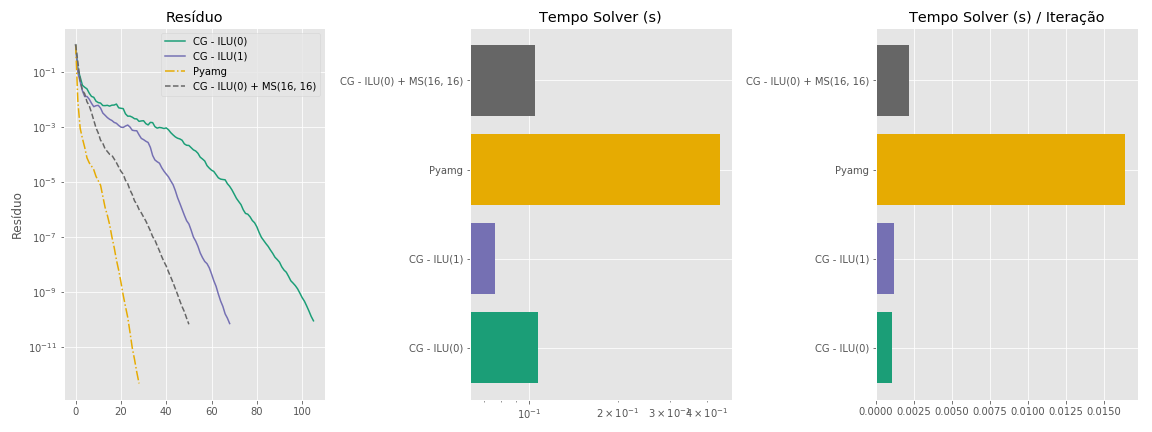
\includegraphics[width=\textwidth]{chap08/figs/reservatorio100x100_2.png}
\caption{Resultados para caso A. Histórico do resíduo relativo ao longo das iterações, tempo do solver em segundos, número de iterações em função do fator de engrossamento da malha e tempo do solver por iteração. }
\label{fig:reservatorio100x100_2}
\end{figure}

Na figura \ref{fig:reservatorio100x100_2} é apresentado a comparação da solução do sistema utilizando o melhor método multiescala com o gradiente conjugado utilizando como precondicionador o ILU(0), ILU(1) e solver multigrid Pyamg. Pode-se notar que apesar da redução de iterações dos método multiescala e do método multigrid, os pré-condicionadores ILU(0) e ILU(1) são mais eficientes na resolução do sistema. 


As figuras \ref{fig:reservatorio320x320_1} e \ref{fig:reservatorio320x320_2} apresentam os mesmos resultados para o caso B.
O engrossamento multiescala de 20x20 é o que resolve o solver em menor tempo, conseguindo inclusive superar o tempo de solução com o solver pré-condicionador ILU(1). O tempo de solução com MS+ILU(1) tem uma melhora de 11,4\% em relação ao tempo do ILU(0). Quando comparado MS+ILU(1) contra ILU(1) o tempo de execução é 45,7\% tempo menor.Além disso, o Pyamg não conseguiu convergir para a solução do problema, parando a execução quando o resíduo atingiu a casa dos $10^{-3}$


\begin{figure}[!htbp]
\centering
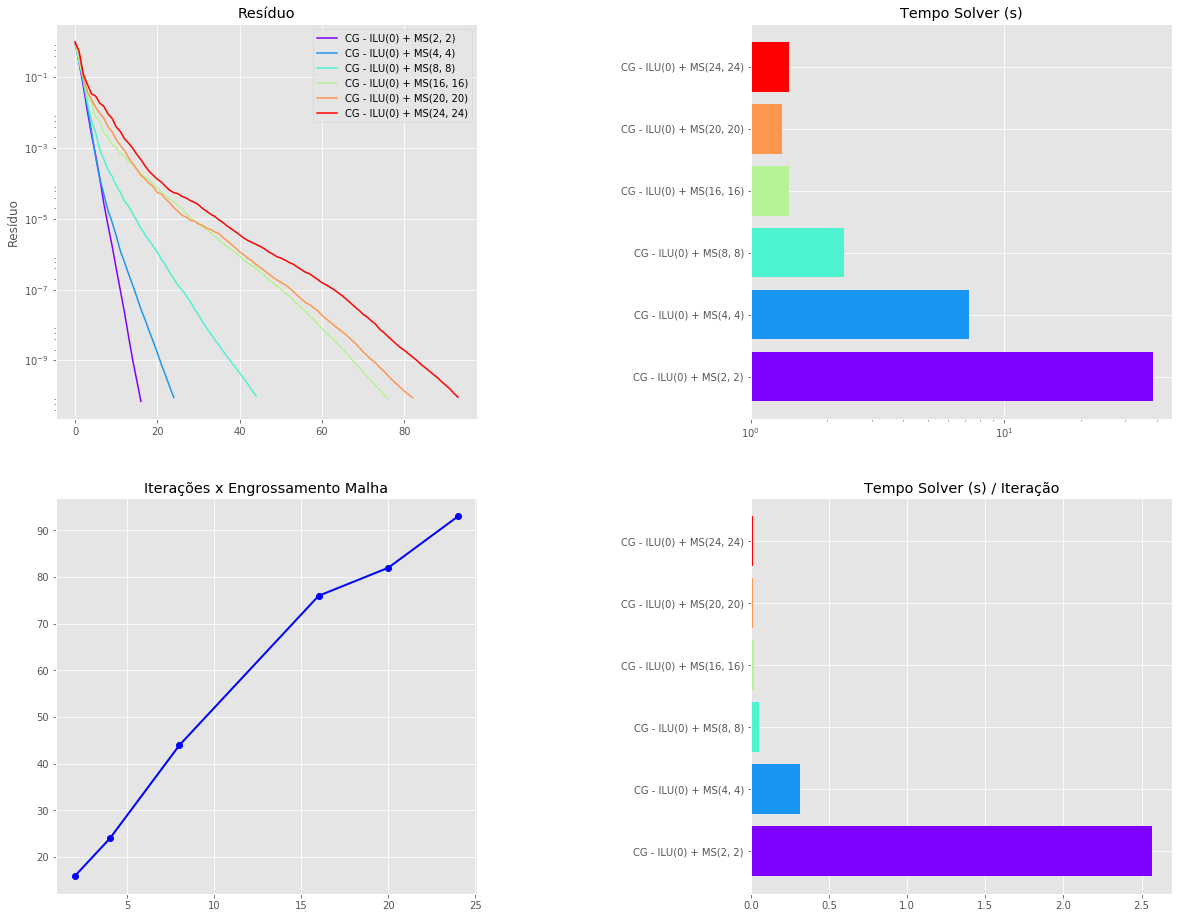
\includegraphics[width=\textwidth]{chap08/figs/reservatorio320x320_1.png}
\caption{Resultados para caso B. Histórico do resíduo relativo ao longo das iterações, tempo do solver em segundos, número de iterações em função do fator de engrossamento da malha e tempo do solver por iteração. }
\label{fig:reservatorio320x320_1} 
\end{figure}


\begin{figure}[!htbp]
\centering
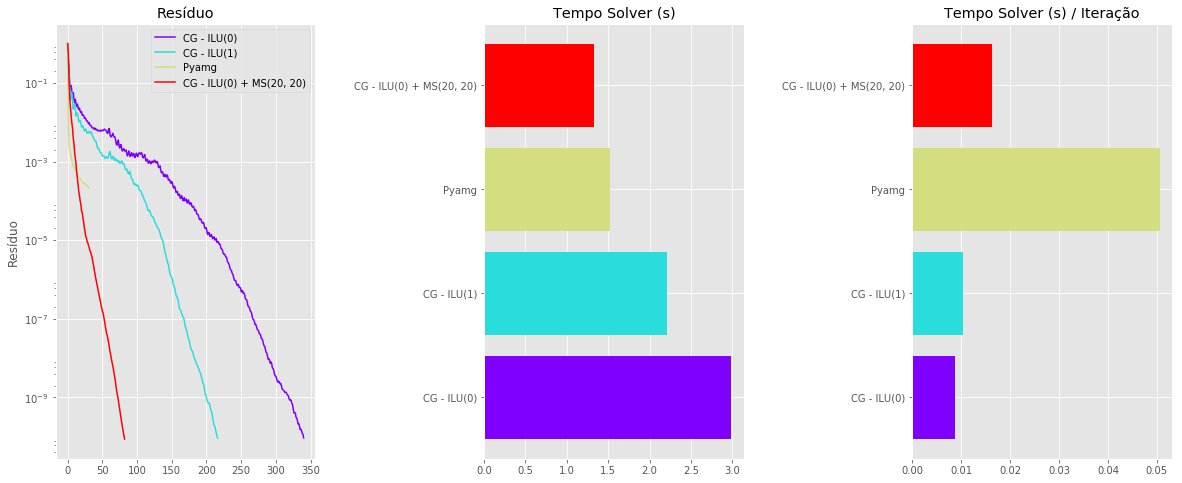
\includegraphics[width=\textwidth]{chap08/figs/reservatorio320x320_2.png}
\caption{Resultados para caso B. Histórico do resíduo relativo ao longo das iterações, tempo do solver em segundos, número de iterações em função do fator de engrossamento da malha e tempo do solver por iteração. }
\label{fig:reservatorio320x320_2}
\end{figure}


A seguir, as figuras \ref{fig:casoC_2}, \ref{fig:casoD_2} e \ref{fig:casoE_2} apresentam os resultados para os casos C, D e E. 
Em todos os gráficos é mostrado apenas o pré-condicionador multiescala que obteve o melhor desempenho entre os fatores de engrossamento de 2x2, 4x4, 8x8, 16x16, 32x32. e é mostrada apenas uma comparação entre os pré-condicionadores multiescala, pyamg, ILU(0) e ILU(1).

\begin{figure}[!htbp]
\centering

\includegraphics[width=6cm]{interrogacao.png}
\caption{Comparação entre multiescala, multigrid e pré-condicionador ILU para o caso C. Histórico do resíduo relativo ao longo das iterações, tempo do solver em segundos e tempo do solver por iteração. }
\label{fig:casoC_2}
\end{figure}

\begin{figure}[!htbp]
\centering
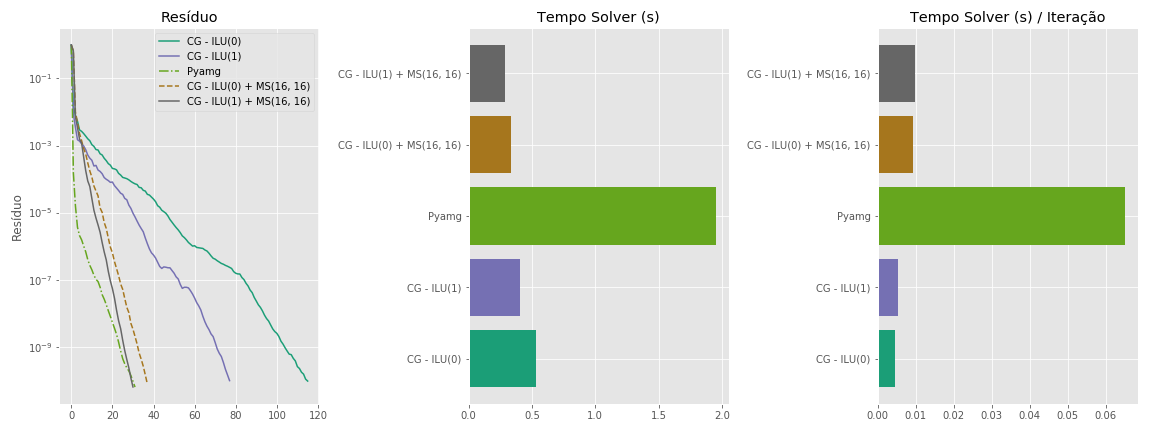
\includegraphics[width=\textwidth]{chap08/figs/casoD_2.png}
\caption{Comparação entre multiescala, multigrid e pré-condicionador ILU para o caso D. Histórico do resíduo relativo ao longo das iterações, tempo do solver em segundos e tempo do solver por iteração. }
\label{fig:casoD_2}
\end{figure}

    
\begin{figure}[!htbp]
\centering
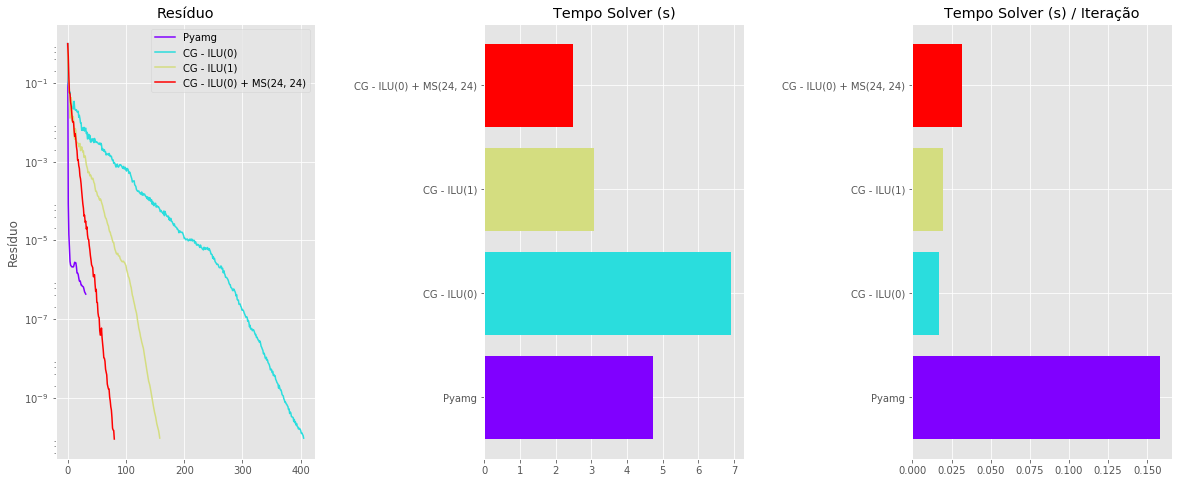
\includegraphics[width=\textwidth]{chap08/figs/casoE_2.png}
\caption{Comparação entre multiescala, multigrid e pré-condicionador ILU para o caso E. Histórico do resíduo relativo ao longo das iterações, tempo do solver em segundos e tempo do solver por iteração. }
\label{fig:casoE_2}
\end{figure}


\subsection{Acurácia da solução grossa}

Nos resultados mostrados nas seções anteriores, era utilizado um solver direto para resolver o sistema grosso. Em casos que a malha foi suficientemente reduzida esse tempo de solução é desprezível, porém, para casos o fator de engrossamento é pequeno resolver exatamente o nível grosso aumenta o tempo de execução (por exemplo, o caso ILU(1) + MS(4,4) em \ref{fig:reservatorio100x100_1}). Além disso, caso modelos muito refinados sejam utilizados o espaço grosseiro pode continuar grande e precise ser resolvido com métodos iterativos, como, por exemplo, para soluções de casos com centenas de milhões de elementos como o mostrado em \cite{geomecrio}.

A avaliação foi feita da seguinte maneira: foi avaliada a quantidade de iterações para resolver o sistema linear com tolerância de $10{-6}$ utilizando o pré-condicionador multiescala com solver do espaço grosso um gradiente conjugado com tolerância variando de $10^{-10}$  a $10^{-1}$. A Figura \ref{fig:toleranciaGrossa} apresenta a quantidade de iterações realizada pelo grid grosso bem como o tempo de execução do solver em cada um dos casos. 


\begin{figure}[!htbp]
\caption{ Variação do número de iterações com tolerância do grid grosso. }
\label{fig:toleranciaGrossa}
\centering

\includegraphics[width=6cm]{interrogacao.png}
\end{figure}


  \chapter{Conclusão e Trabalhos Futuros}

  \backmatter
  \nocite{*}
  \bibliographystyle{coppe-unsrt}
  \bibliography{thesis}
  \appendix
  \chapter{Figuras dos reservatórios} \label{ch:figurasReservatorios}

Aqui estão apresentadas os grids dos casos C, D e E que foram utilizados para a exposição dos resultados.
As escalas dos casos D e E foram omitidas por se tratarem de modelos reais e os dados, portanto, são sensíveis para a Petrobras.



\begin{figure}[h]
\center
\subfigure[ ]{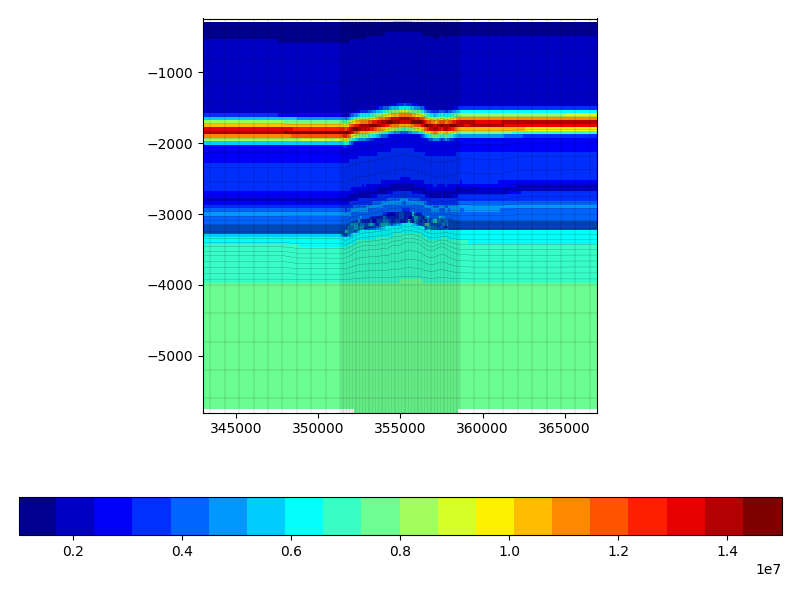
\includegraphics[width=0.45\textwidth]{append/figs/pituba_young.png}}
\qquad
\subfigure[ ]{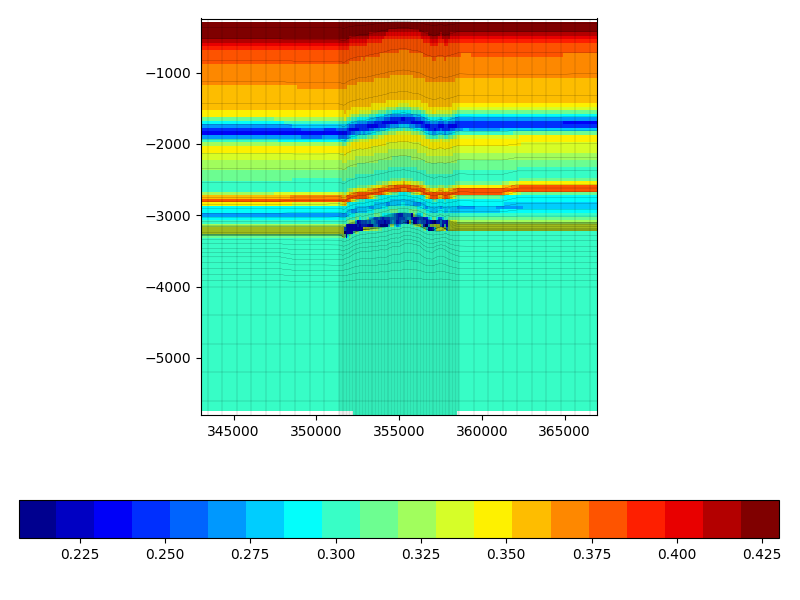
\includegraphics[width=0.45\textwidth]{append/figs/pituba_poisson.png}}
\caption{Propriedades módulo de Young (a) e coeficiente de poisson (b) para caso C } \label{fig:casoCgrid}
\end{figure}

\begin{figure}[h]

\center
\subfigure[ ]{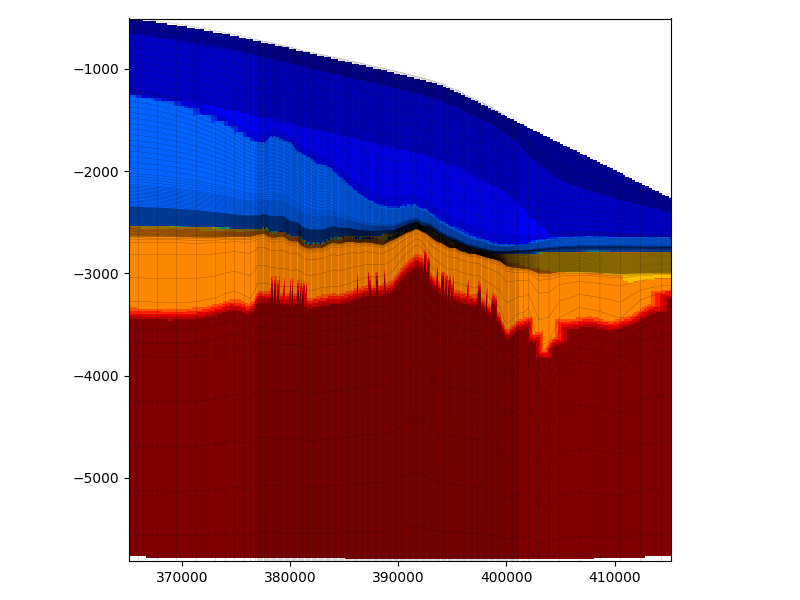
\includegraphics[width=\textwidth]{append/figs/refined_young.png}}
\qquad
\subfigure[ ]{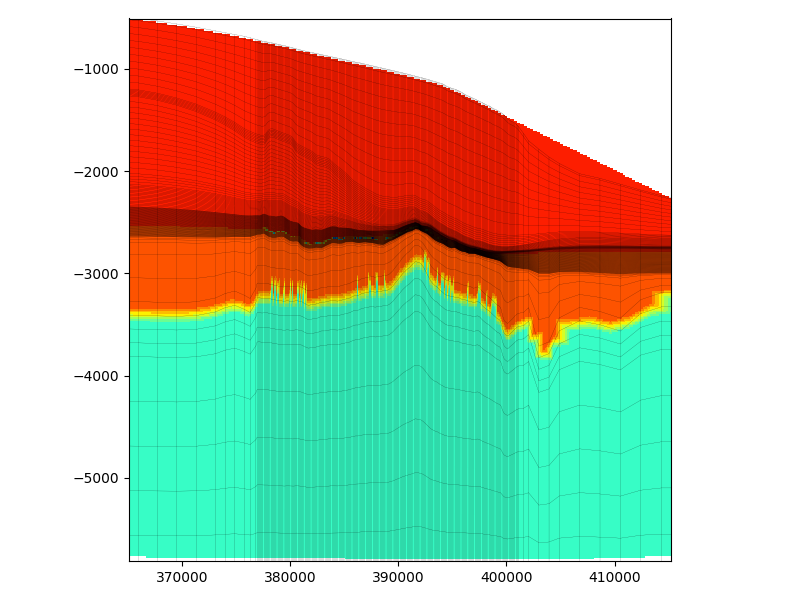
\includegraphics[width=\textwidth]{append/figs/refined_poisson.png}}
\caption{Propriedades módulo de Young (a) e coeficiente de poisson (b) para caso D } \label{fig:casoDgrid}
\end{figure}





\begin{figure}[h]
\center
\subfigure[ ]{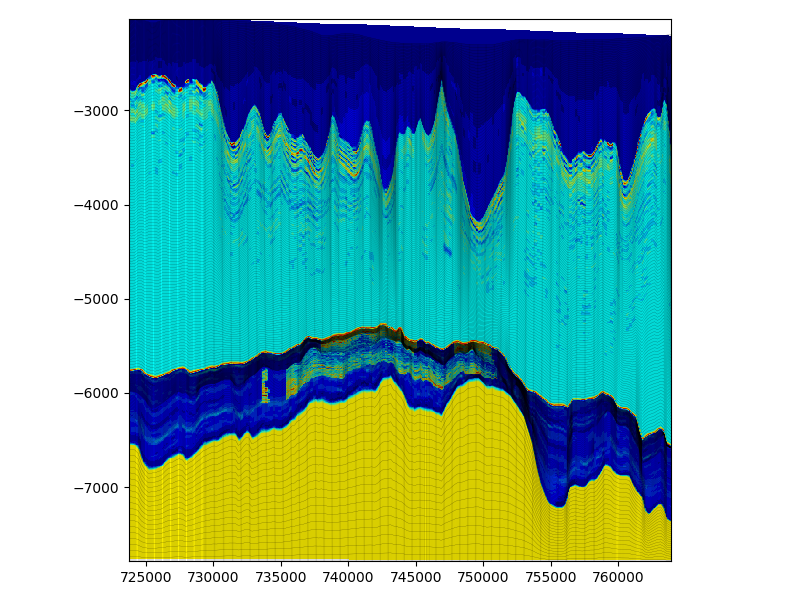
\includegraphics[width=\textwidth]{append/figs/93MM_young.png}}
\qquad
    \subfigure[ ]{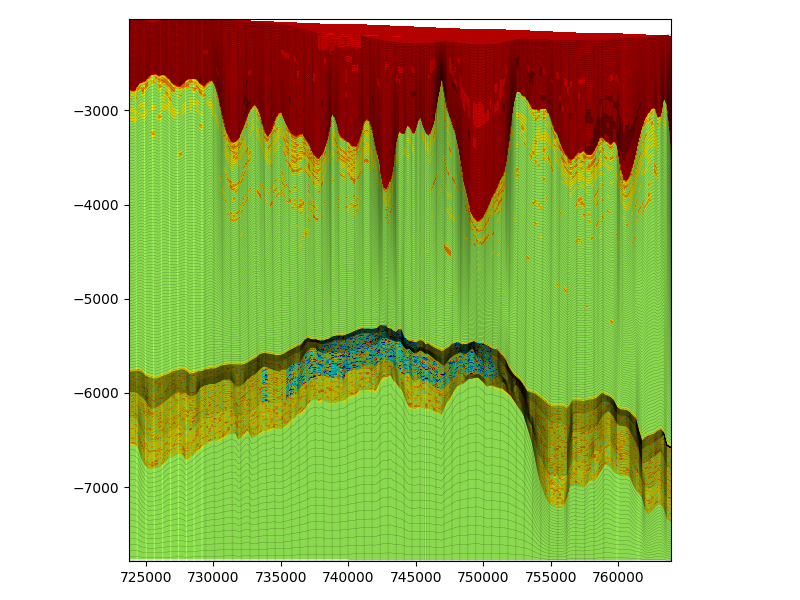
\includegraphics[width=\textwidth]{append/figs/93MM_poisson.png}}
\caption{Propriedades módulo de Young (a) e coeficiente de poisson (b) para caso E } \label{fig:casoEgrid}
\end{figure}


\begin{figure}[h]
\center
\subfigure[ ]{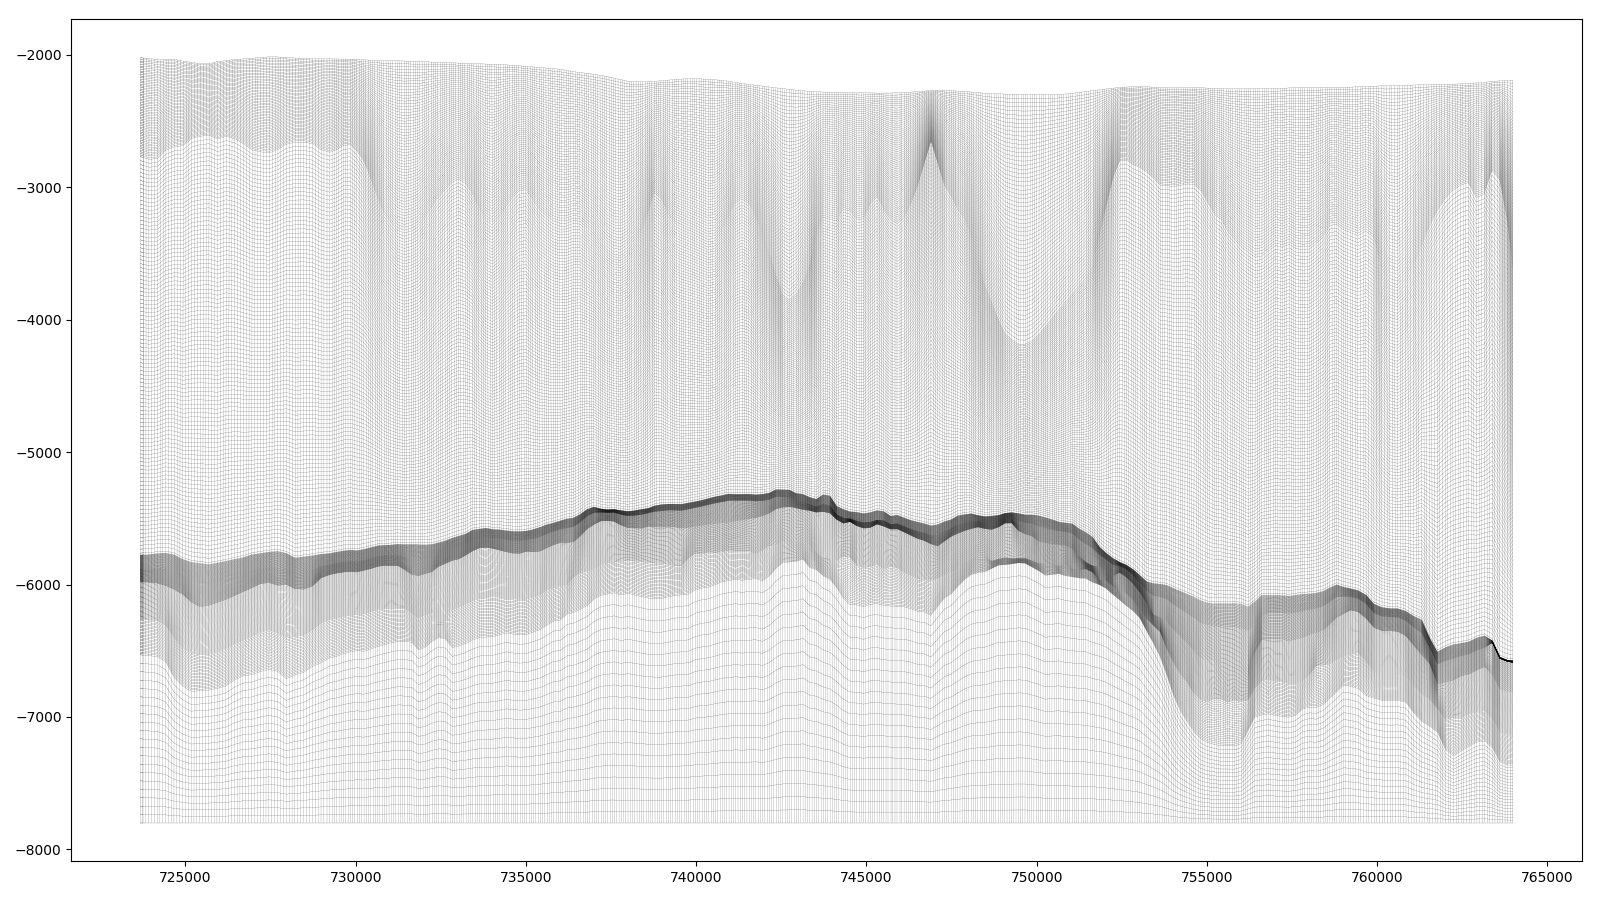
\includegraphics[width=\textwidth]{append/figs/93MM_grid.png}}
\qquad
\subfigure[ ]{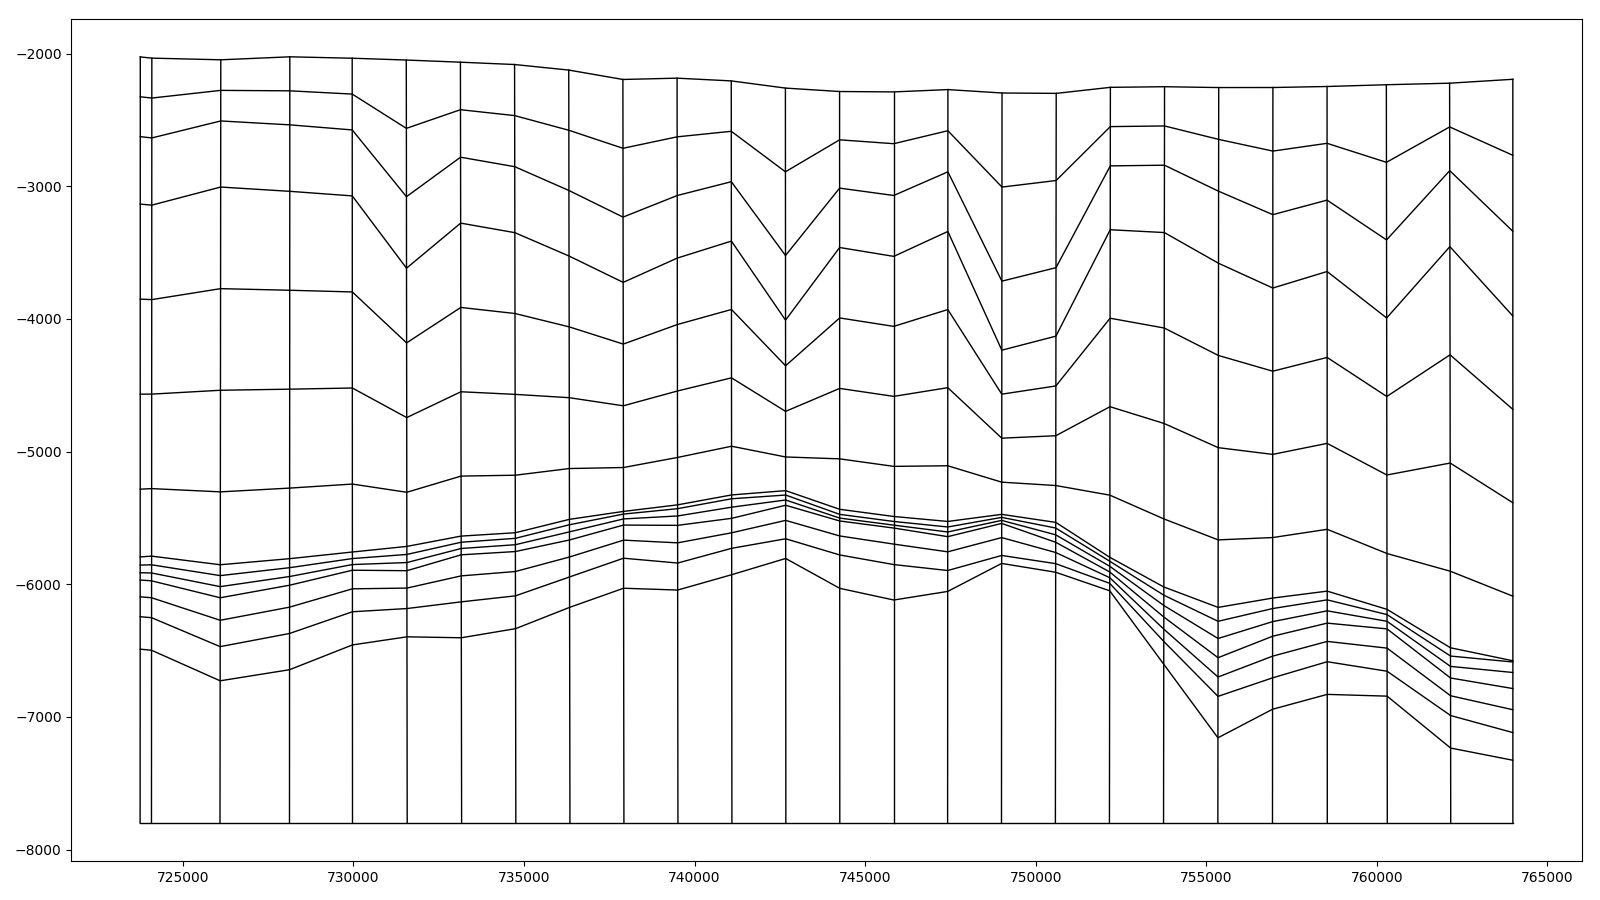
\includegraphics[width=\textwidth]{append/figs/93MM_24x24.png}}
\caption{Grid de simulação original (a) e após refinamento 24 x 24(b) para caso E } \label{fig:casoEgrid_figures}
\end{figure}

  \chapter{Configurações de solver utilizadas pelo Pyamg} \label{ch:pyamgSolver}


Seguem abaixo as chamadas com os parâmetros para construção dos solvers multigrid  utilizados pelo PyAMG para os resultados apresentados no Capítulo \ref{ch:resultados}. Esses foram retornados pelo script \textbf{solver\_diagnostics.py}. Em todos os casos a chamada do solver multigrid foi sugerida com o ciclo W e como pré-condicionador para o Gradiente Conjugado. 


\subsubsection{Caso A e Caso B}

\begin{lstlisting}[
    basicstyle=\small, %or \small or \footnotesize etc.
]
smoothed_aggregation_solver(A, B=B, BH=BH,
  strength=('evolution', {'k': 2, 'proj_type': 'l2', 'epsilon': 2.0}),
  smooth=('energy', {'krylov': 'cg', 'maxiter': 2, 
          'degree': 1, 'weighting': 'local'}),
  improve_candidates=[('block_gauss_seidel', 
                      {'sweep': 'symmetric', 'iterations': 4}), 
                      None, None, None, None, None, None,
                      None, None, None, None, None,
                      None, None, None],
  aggregate="standard",
  presmoother=('block_gauss_seidel', 
               {'sweep': 'symmetric', 'iterations': 1}),
  postsmoother=('block_gauss_seidel', 
                {'sweep': 'symmetric', 'iterations': 1}),
  max_levels=15,
  max_coarse=300,
  coarse_solver="pinv")
\end{lstlisting}

\subsubsection{Caso C}

\begin{lstlisting}[
    basicstyle=\small, %or \small or \footnotesize etc.
]
smoothed_aggregation_solver(A, B=B, BH=BH,
  strength=('evolution', {'k': 2, 'proj_type': 'l2', 'epsilon': 2.0}),
  smooth=('energy', {'krylov': 'cg', 'maxiter': 2, 
                     'degree': 1, 'weighting': 'local'}),
  improve_candidates=[('block_gauss_seidel', 
                      {'sweep': 'symmetric', 'iterations': 4}), 
                      None, None, None, None, None, None, None, 
                      None, None, None, None, None, None, None],
  aggregate="standard",
  presmoother=('block_gauss_seidel', 
               {'sweep': 'symmetric', 'iterations': 1}),
  postsmoother=('block_gauss_seidel', 
                {'sweep': 'symmetric', 'iterations': 1}),
  max_levels=15,
  max_coarse=300,
  coarse_solver="pinv")
\end{lstlisting}


\subsubsection{Caso D e Caso E}

\begin{lstlisting}[
    basicstyle=\small, %or \small or \footnotesize etc.
]
smoothed_aggregation_solver(A, B=B, BH=BH,
  strength=('evolution', {'k': 2, 'proj_type': 'l2', 'epsilon': 2.0}),
  smooth=('energy', {'krylov': 'cg', 'maxiter': 2, 
                     'degree': 1, 'weighting': 'local'}),
  improve_candidates=None,
  aggregate="standard",
  presmoother=('block_gauss_seidel', 
               {'sweep': 'symmetric', 'iterations': 1}),
  postsmoother=('block_gauss_seidel', 
                {'sweep': 'symmetric', 'iterations': 1}),
  max_levels=15,
  max_coarse=300,
  coarse_solver="pinv")
\end{lstlisting}

\end{document}
